\documentclass[xcolor=pdftex,dvipsnames,table,10pt,babel,spanish]{beamer}

\usetheme{Warsaw}


\usepackage[spanish]{babel}
\usepackage[latin1]{inputenc}
\usepackage{stmaryrd}
\usepackage{graphicx}
\usepackage{wrapfig}
\usepackage{listings}

\usepackage{setspace}

\usepackage{color}
\usepackage{textcomp}
\definecolor{listinggray}{gray}{0.9}
\definecolor{lbcolor}{rgb}{0.95,0.95,0.95}
\lstset{
    backgroundcolor=\color{lbcolor},
    tabsize=4,6
    rulecolor=,
    language=matlab,
        basicstyle=\scriptsize,
        upquote=true,
        aboveskip={1.5\baselineskip},
        columns=fixed,
        showstringspaces=false,
        extendedchars=true,
        breaklines=true,
        prebreak = \raisebox{0ex}[0ex][0ex]{\ensuremath{\hookleftarrow}},
        frame=single,
        showtabs=false,
        showspaces=false,
        showstringspaces=false,
        identifierstyle=\ttfamily,
        keywordstyle=\color[rgb]{0.1,0.1,0.6}\bfseries,
        commentstyle=\color[rgb]{0.133,0.545,0.133},
        stringstyle=\color[rgb]{0.627,0.126,0.941},
}
\newcommand{\fudepan}{\textbf{FuDePAN}}
\newcommand{\combeng}{\textbf{CombEng}}
\newcommand{\recabs}{\textbf{RecAbs}}
\newcommand{\rnaffe}{\textbf{RnaFFE}}
\newcommand{\fud}{\textbf{FuD}}

\setbeamercovered{transparent}

\title{Implementation of a Distributed Combinatory Engine}
\subtitle{And its Application to Bioinformatic Problems}
\author{Favio Bettiol \and Diego Diaz}
\pgfdeclareimage[height=2.5cm]{unrc}{images/escudo_unrc.png}
%\pgfdeclareimage[height=2.5cm]{fud}{images/fud_logo.png}
\pgfdeclareimage[height=2.5cm]{fudepan}{images/fudepan.png}

\institute[U.N.R.C.]{
  \textsc{Departamento de Computaci\'on} \\
  \textsc{Universidad Nacional de R\'io Cuarto} \\
  \textsc{y}\\
  \textsc{FuDePAN} \\
  \ \\  
  %\pgfuseimage{unrc}  \qquad \qquad \pgfuseimage{fud} \qquad \qquad \pgfuseimage{fudepan}}

  \pgfuseimage{unrc} \qquad \qquad \pgfuseimage{fudepan}}
\date{}

\begin{document}

\frame{\titlepage}

\frame{
    \frametitle{Acerca de este trabajo}
    Un trabajo coordinado entre la UNRC y \textbf{FuDePAN}, Fundaci\'on para el Desarrollo de la Programaci\'on en \'Acidos Nucleicos.
    \vspace{1cm}
    \begin{block}{}
    Dentro del mismo trabajo, claramente, se distinguen dos proyectos:
    \begin{itemize}
      \item \textbf{La implementaci\'on de un motor combinatorio}.
      \item \textbf{Una aplicaci\'on relevante para la fundaci\'on}.
    \end{itemize}
  \end{block}
}

\frame{
\frametitle{Temario: }
\tableofcontents
}

\section{Motor Combinatorio}
\subsection{Motivaci\'on}
\frame{
    \frametitle{Motivaci\'on}
    \textbf{FuDePAN} necesitaba contar con un motor combinatorio debido a la gran cantidad de problemas, de caracter bioinform\'atico, que se ven
    caracterizados por:    
        \begin{itemize}
            \item Requerir un motor combinatorio para la generaci\'on de \'arboles de combinaciones.
            \item Utilizar mecanismos de poda sobre dichos \'arboles.
            \item Requerir un sistema de puntuaci\'on por cada una de las combinaciones (\textit{ranking} o \textit{scoring}).
        \end{itemize}
%      \vspace{.5cm}
    \pause
    \begin{block}{}
      Debido a que la gran cantidad de problemas tienen como caracter\'istica com\'un requerir un elevado nivel de c\'omputo, 
      se opt\'o por implementar al motor combinatorio como una nueva capa sobre un framework para aplicaciones distribuidas, llamado \textbf{FuD}.
    \end{block}
}

\subsection{Marco Te\'orico}
\subsubsection{FuD}
\frame{
  \frametitle{El framework \textbf{FuD}}
    \textbf{FuD} (\textbf{F}uDePAN \textbf{U}biquitous \textbf{D}istribution) es un framework para automatizar la distribuci\'on de
    aplicaciones computacionales a trav\'es de disposiciones heterog\'eneas y din\'amicas de nodos de procesamiento.

    \begin{block}{Ventajas de utilizar \textbf{FuD}}
      \begin{itemize}
        \item Debe poder ser utilizado para resolver cualquier problema que se puede solucionar secuencialmente.
        \item No requiere que el usuario del framework:
          \begin{itemize}
            \item Sepa conceptos de programaci\'on paralela.
            \item Quede restringido a una determinada disposici\'on de nodos procesadores.
            \item Quede limitado por un particular sistema de comunicaci\'on.
          \end{itemize}
      \end{itemize}
    \end{block}
}

\frame{
  \frametitle{El framework \textbf{FuD} \small{(Cont.)}}
  Por otra parte, \textbf{FuD} asegura:
    \begin{itemize}
      \item Que la aplicaci\'on implementada tiene el potencial de ejecutarse paralelamente.
%      \pause
      \item Que la aplicaci\'on explotar\'a los recursos que se pongan a su disposici\'on.
%      \pause
      \item El uso del framework no generar\'a p\'erdidas de performance considerables.
%      \pause
      \item Los datos intercambiados entre aplicaciones cliente y servidor no llevar\'an una carga adicional significativa sobre los datos
      necesarios para la aplicaci\'on.
    \end{itemize}
}

\frame{
  \frametitle{El framework \textbf{FuD} \small{(Cont.)}} 
     \begin{center}
        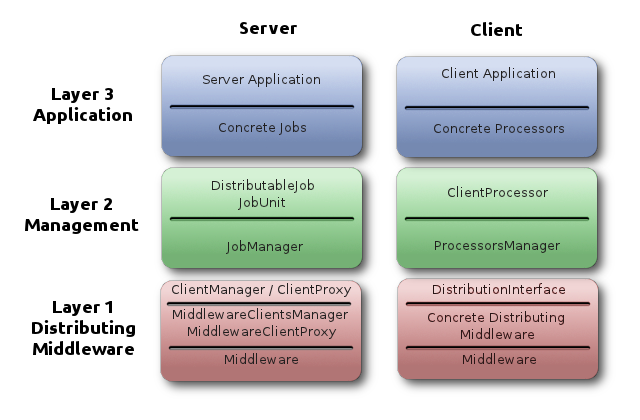
\includegraphics[scale=.45]{images/AbstractLayers.png}
      \end{center}
}

\frame{
  \frametitle{Capas del framework}
    El framework combina los conceptos de Cliente-Servidor y Divide \& Conquer. Adem\'as, presenta una estructuraci\'on en capas:
    \begin{description}
    \item[Aplicaci\'on]: Esta capa provee componentes que contienen todos los aspectos del dominio del problema. Como tal, incluye las definiciones
      y manejo de los datos usados y el algoritmo relevante a la soluci\'on implementada.
%    \pause
    \item[Manejo de trabajo]: Esta capa se encarga de manejar ambos tipos de trabajo, haciendo de nexo entre la aplicaci\'on, donde se encuentran
      los trabajos concretos y se producen las unidades de trabajo, y los clientes, que se manejan en la capa inferior.
%    \pause
    \item[Comunicaci\'on]: En esta capa existe el \'unico v\'inculo real entre clientes y servidor, la responsabilidad de esta capa es manejar los
      clientes conectados al servidor y llevar acabo los procedimientos de comunicaci\'on entre ambas aplicaciones.        
    \end{description}
}
\subsection{Dise\~no}
\frame{
    \frametitle{?`Qu\'e es \textbf{CombEng}?}
    Es una nueva capa sobre el framework \textbf{FuD}, respetando el modelo Cliente-Servidor. \textbf{CombEng} no depende del problema a ser
    implementado, sino que define una estructura com\'un para implementar la soluci\'on aquellos problemas que requieren de un motor combinatorio.
    \vspace{-.2cm}
     \begin{center}
        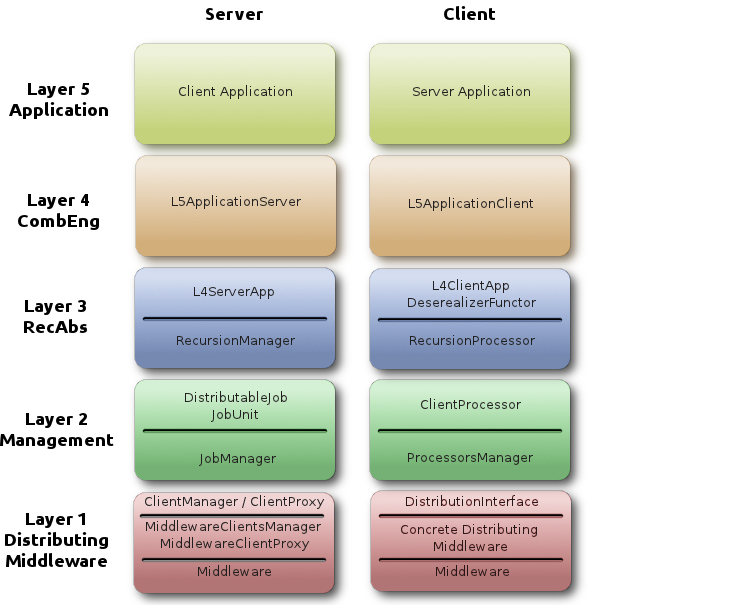
\includegraphics[scale=.27]{images/AbstractLayersRedesigned.png}
      \end{center}
}

\frame{
    \frametitle{?`Qu\'e es \textbf{CombEng}?}
    Es una nueva capa sobre el framework \textbf{FuD}, respetando el modelo Cliente-Servidor. \textbf{CombEng} no depende del problema a ser
    implementado, sino que define una estructura com\'un para implementar la soluci\'on aquellos problemas que requieren de un motor combinatorio.
    \vspace{-.2cm}
     \begin{center}
        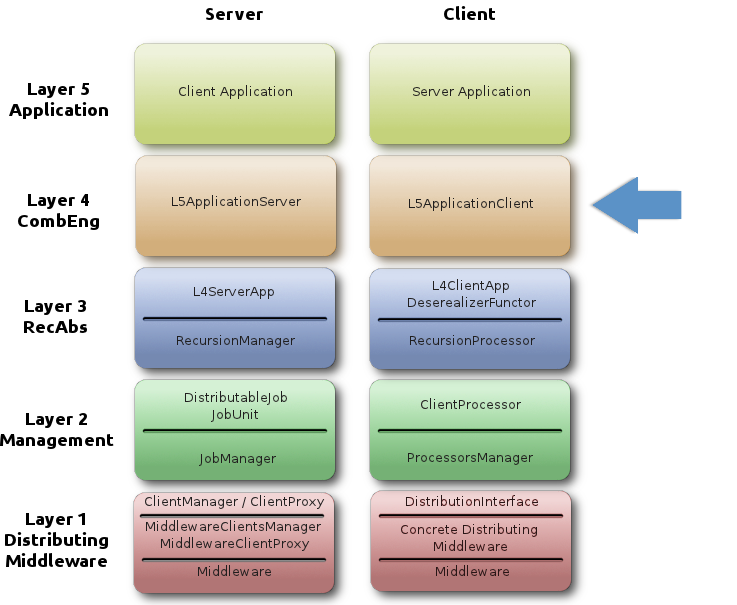
\includegraphics[scale=.27]{images/AbstractLayersRedesigned2.png}
      \end{center}
}

\frame{
    \frametitle{Diagrama de Clases}
    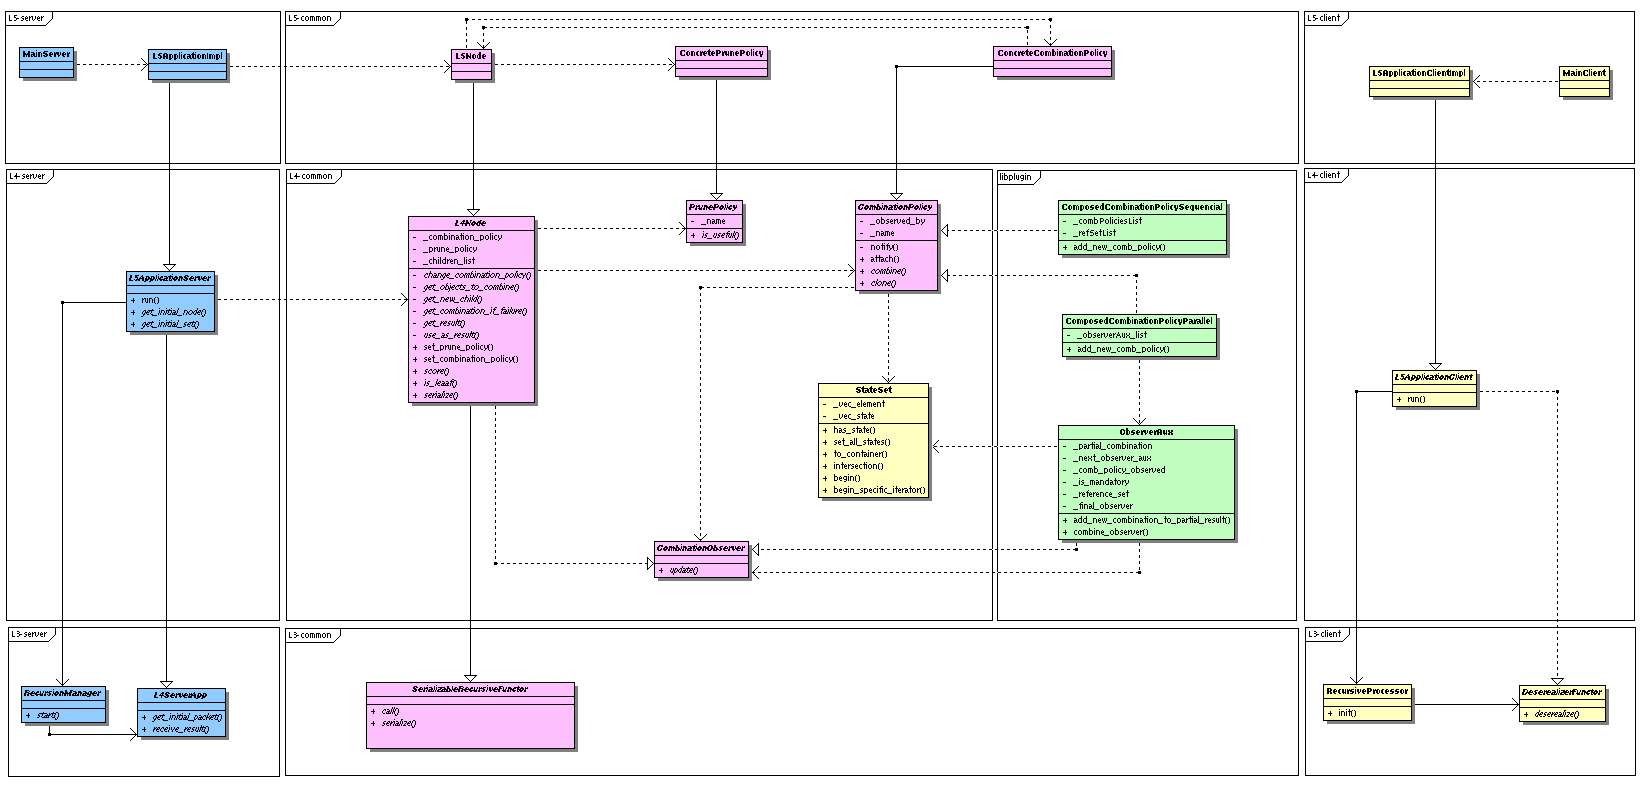
\includegraphics[scale=.2]{images/classDiagram.png}
}

\subsubsection{Lado Servidor}
\frame{
    \frametitle{Diagrama de Clases - Lado Servidor}
    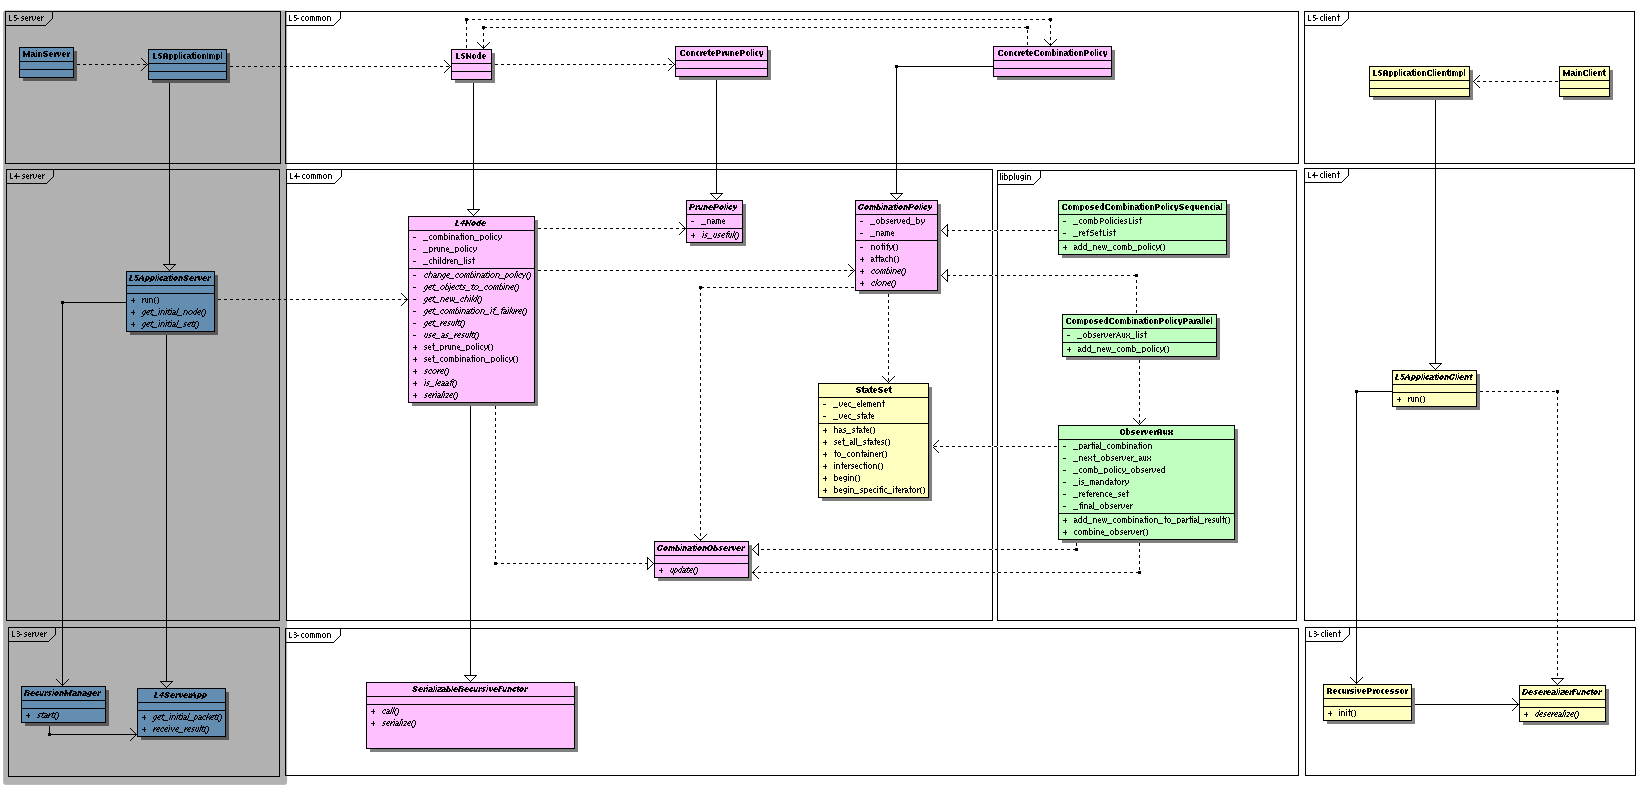
\includegraphics[scale=.2]{images/serverSide.png}
}

\frame{
\frametitle{Lado Servidor}
\begin{figure}[h]
  \begin{minipage}{4cm}
    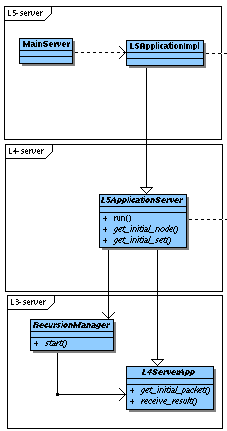
\includegraphics[scale=.4]{images/server.png}
  \end{minipage}
  \begin{minipage}{0.6 \textwidth} % 0.5 \textwidth = 50% ancho de página
    Constituye la aplicaci\'on \textit{Servidor}.\\
    Sus principales tareas son:
    \begin{itemize}
      \item Generar unidades de trabajo.
%      \item Ejecutar la aplicaci\'on \textit{Servidor}.
%        \begin{itemize}
%          \item Obtener el nodo inicial\\(nodo ra\'iz del \'arbol).
%          \item Conjunto inicial de elementos que se requieren combinar.
%        \end{itemize}
      \item Asignar trabajo a los clientes conectados.
      \item Recolectar y procesar datos provenientes de los clientes.
      \item Informar resultados.
    \end{itemize}
  \end{minipage}
\end{figure}
}

\subsubsection{Lado Cliente}
\frame{
    \frametitle{Diagrama de Clases - Lado Cliente}
    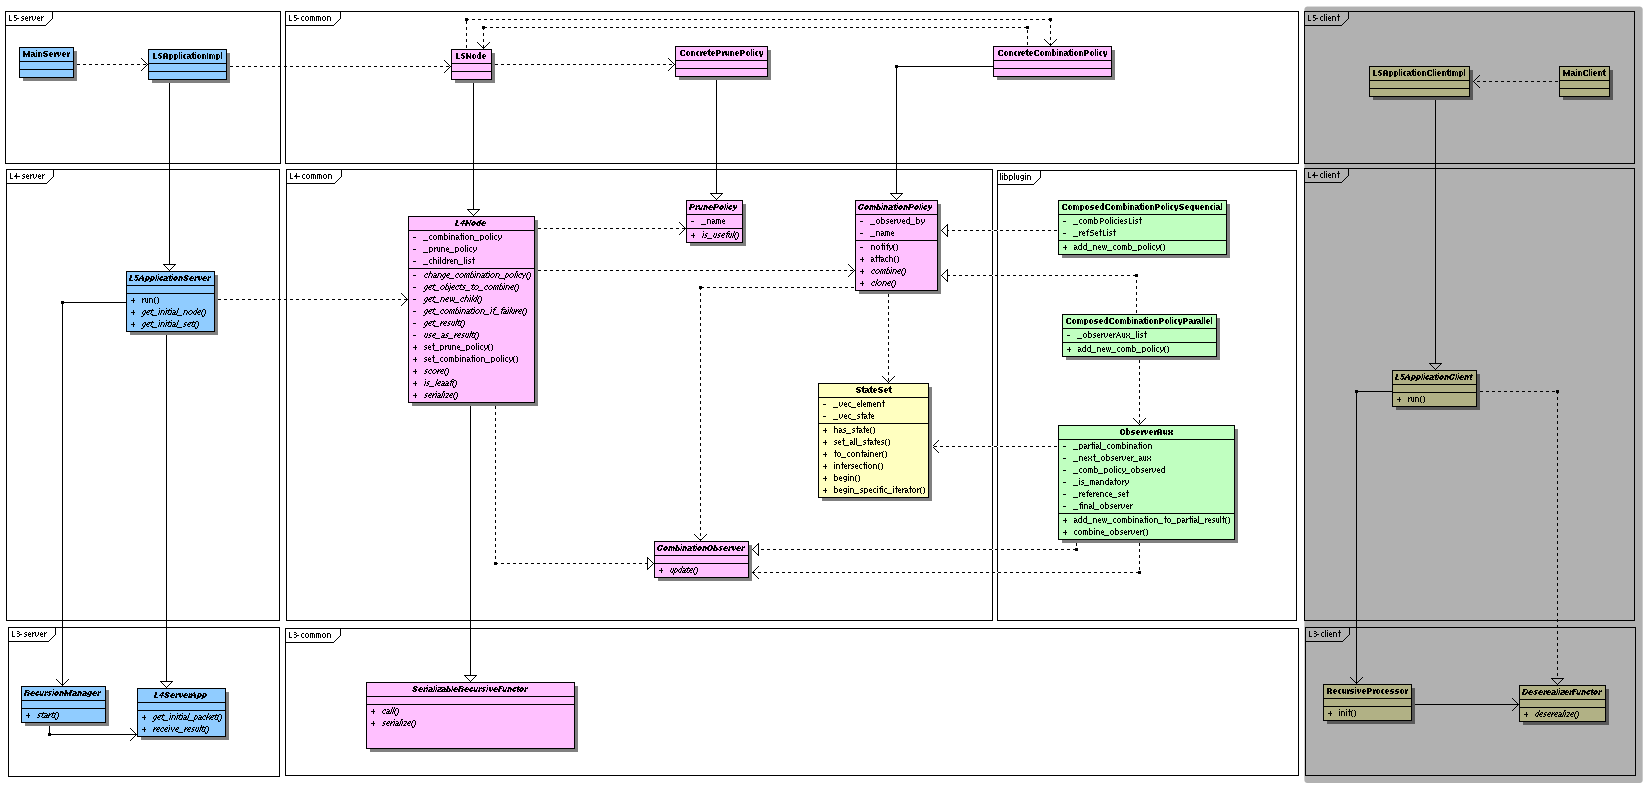
\includegraphics[scale=.2]{images/clientSide.png}
}

\frame{
  \frametitle{Lado Cliente}
  \begin{figure}[h]
    \begin{minipage}{4cm}
      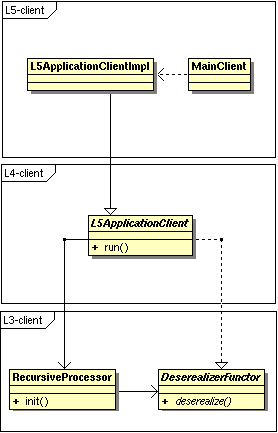
\includegraphics[width=40mm,height=70mm]{images/client.png}
    \end{minipage}
    \begin{minipage}{0.6 \textwidth}
      Constituye la aplicaci\'on \textit{Cliente}.\\
      Sus principales tareas son:
      \begin{itemize}
        \item Recibir un trabajo asignado por la aplicaci\'on servidor.
        \item Procesar dicho trabajo.
        \item Enviar los resultados parciales de regreso.
      \end{itemize}
    \end{minipage}
  \end{figure}
}
\subsubsection{Lado Com\'un}
\frame{
    \frametitle{Diagrama de Clases - Lado Com\'un}
    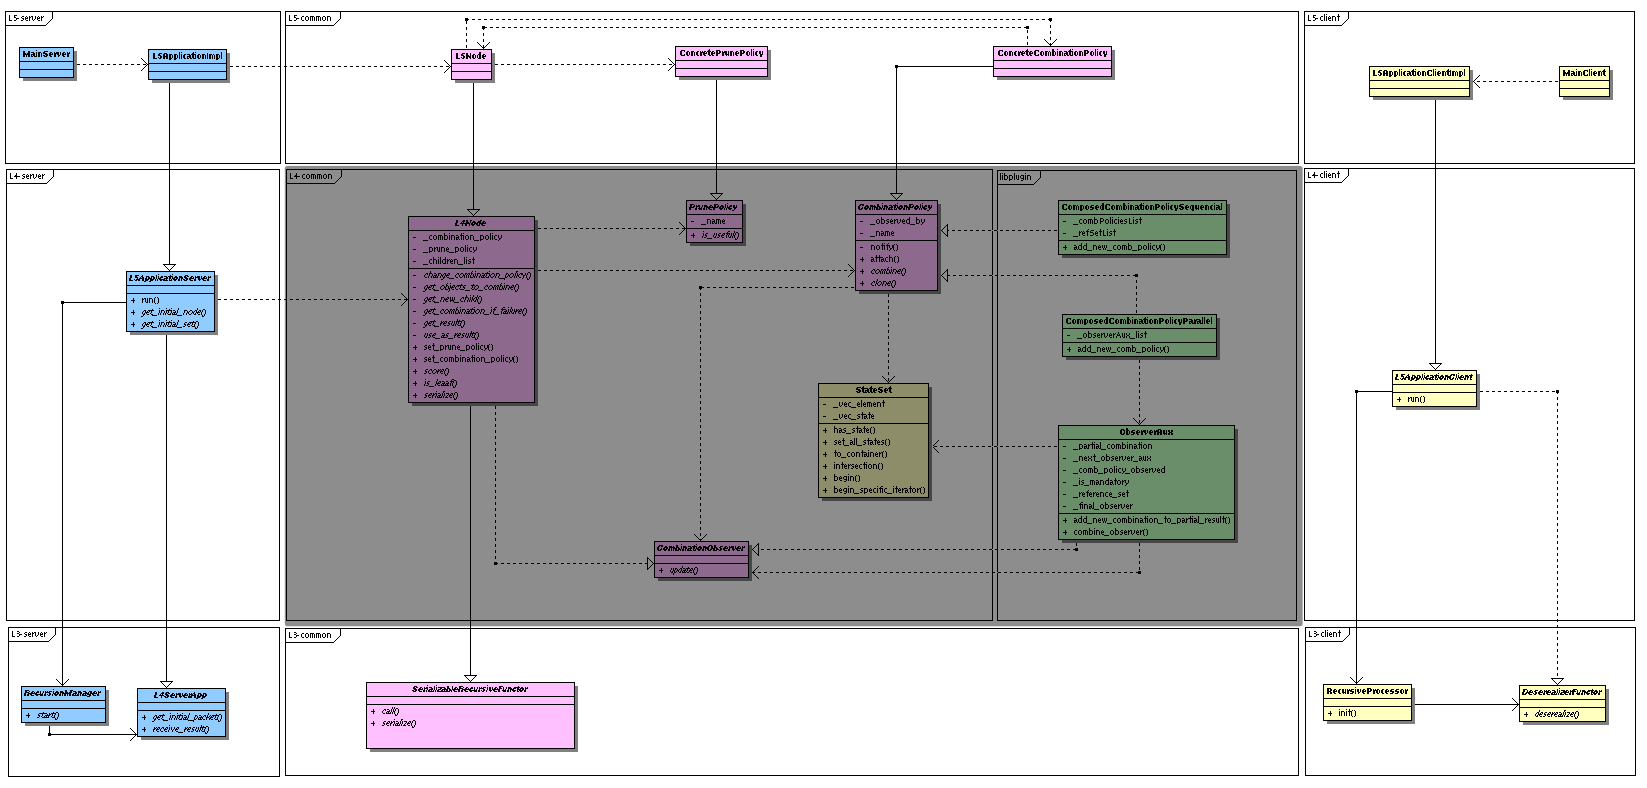
\includegraphics[scale=.2]{images/commonSide.png}
}

\frame{
  \frametitle{Lado Com\'un}
  \begin{figure}[H]
    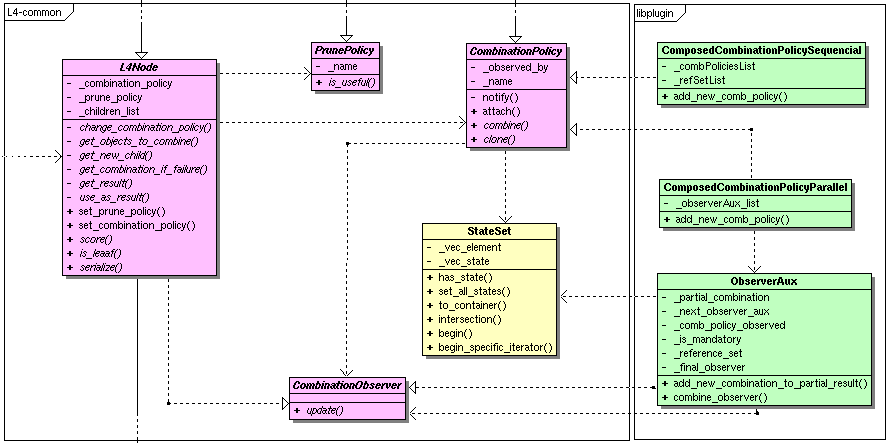
\includegraphics[scale=.35]{images/commonZoom.png}
  \end{figure}
}

\subsubsection{Pol\'iticas de Combinaci\'on}
\frame{
  \frametitle{Lado Com\'un}
  \begin{block}{Pol\'iticas de combinaci\'on}
  Una pol\'itica de combinaci\'on define la forma en que una colecci\'on de elementos ser\'a combinada.
  Su dise\~no responde al patr\'on \textit{Observer}:
  \begin{itemize}
    \item La pol\'itica es un objeto observable.
    \item La pol\'itica notifica, a los objetos que la observan, que una nueva combinaci\'on ha sido generada.
  \end{itemize}
  \end{block}
  \begin{block}{}
    Como parte de este trabajo, se han implementado diferentes pol\'iticas de combinaci\'on, algunas \textbf{simples} y otras \textbf{compuestas}.
  \end{block}
}

\frame{
  \frametitle{Lado Com\'un}
  \textbf{Pol\'iticas simples}\\
    Son algoritmos combinadores propiamente dichos.
    \begin{exampleblock}{Pol\'iticas simples implementadas}
      \begin{itemize}
        \item \texttt{ListCombinationPolicy}: retorna uno a uno los elementos a combinar.
        \item \texttt{NewtonianCombinationPolicy}: implementa el cl\'asico algoritmo que retorna todos los subconjuntos de tama\~no K, 
          con \emph{MIN$\leq$K$\geq$MAX}.

          Por ejemplo, con \textbf{K = 2}:
          \vspace{-.5cm}
          \begin{center}
            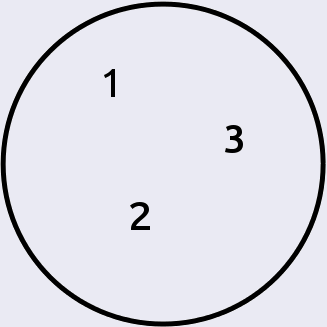
\includegraphics[scale=.25]{images/newtonian.png}
          \end{center}
      \end{itemize}
    \end{exampleblock}
}

\frame{
  \frametitle{Lado Com\'un}
  \textbf{Pol\'iticas simples}\\
    Son algoritmos combinadores propiamente dichos.
    \begin{exampleblock}{Pol\'iticas simples implementadas}
      \begin{itemize}
        \item \texttt{ListCombinationPolicy}: retorna uno a uno los elementos a combinar.
        \item \texttt{NewtonianCombinationPolicy}: implementa el cl\'asico algoritmo que retorna todos los subconjuntos de tama\~no K, 
          con \emph{MIN$\leq$K$\geq$MAX}.

          Por ejemplo, con \textbf{K = 2}:
          \vspace{-.5cm}
          \begin{center}
            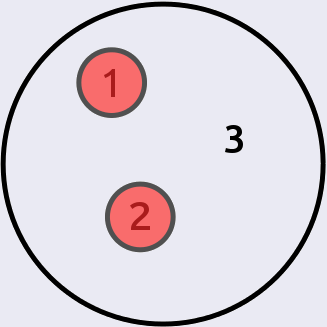
\includegraphics[scale=.25]{images/newtonian1.png}
          \end{center}
      \end{itemize}
    \end{exampleblock}
}

\frame{
  \frametitle{Lado Com\'un}
  \textbf{Pol\'iticas simples}\\
    Son algoritmos combinadores propiamente dichos.
    \begin{exampleblock}{Pol\'iticas simples implementadas}
      \begin{itemize}
        \item \texttt{ListCombinationPolicy}: retorna uno a uno los elementos a combinar.
        \item \texttt{NewtonianCombinationPolicy}: implementa el cl\'asico algoritmo que retorna todos los subconjuntos de tama\~no K, 
          con \emph{MIN$\leq$K$\geq$MAX}.

          Por ejemplo, con \textbf{K = 2}:
          \vspace{-.5cm}
          \begin{center}
            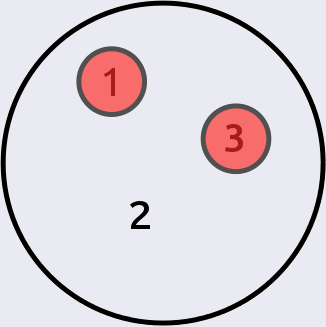
\includegraphics[scale=.25]{images/newtonian2.png}
          \end{center}
      \end{itemize}
    \end{exampleblock}
}

\frame{
  \frametitle{Lado Com\'un}
  \textbf{Pol\'iticas simples}\\
    Son algoritmos combinadores propiamente dichos.
    \begin{exampleblock}{Pol\'iticas simples implementadas}
      \begin{itemize}
        \item \texttt{ListCombinationPolicy}: retorna uno a uno los elementos a combinar.
        \item \texttt{NewtonianCombinationPolicy}: implementa el cl\'asico algoritmo que retorna todos los subconjuntos de tama\~no K, 
          con \emph{MIN$\leq$K$\geq$MAX}.

          Por ejemplo, con \textbf{K = 2}:
          \vspace{-.5cm}
          \begin{center}
            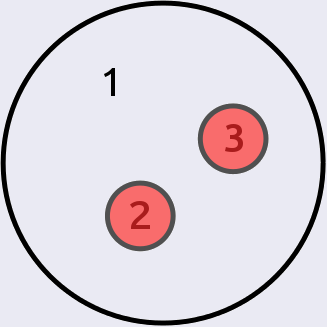
\includegraphics[scale=.25]{images/newtonian3.png}
          \end{center}
      \end{itemize}
    \end{exampleblock}
}

\frame{
  \frametitle{Lado Com\'un}
  \textbf{Pol\'iticas compuestas}\\
  \begin{itemize}
    \item Combinan dos o m\'as pol\'iticas simples.
    \item No generan combinaciones por s\'i mismas, son las simples quienes se encargan de obtenerlas.
  \end{itemize}
  \begin{exampleblock}{Pol\'itica compuesta secuencial}
    Establece una especie de nexo entre diferentes algoritmos combinatorios. B\'asicamente, toma un conjunto de combinadores y los hace combinar
    en secuencia, uno despu\'es de otro. Podr\'ia pensarse como una cola (FIFO) de combinadores, el primero en ingresar a la cola es el primero en combinar.
      \vspace{-.3cm}
	  	\begin{figure}[H]\hspace{.8cm}
	  		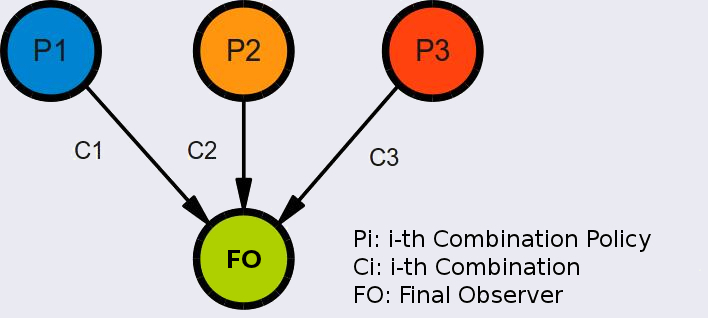
\includegraphics[scale=.25]{images/Comb1.jpg}
	  	\end{figure}
  \end{exampleblock}
}

\frame{
  \frametitle{Lado Com\'un}
  \begin{exampleblock}{Pol\'itica compuesta paralela}
    Toma un grupo de algoritmos combinadores y los pone a ``correr'' en paralelo. Es decir, cada combinaci\'on que genera la primer pol\'itica
    se une con cada combinaci\'on generada por la segunda y as\'i sucesivamente, hasta llegar a la \'ultima de \'estas, la cual har\'a entrega
    de todo el paquete al observador final. \vspace{-.18cm}
		\begin{figure}[H]\hspace{.3cm}
			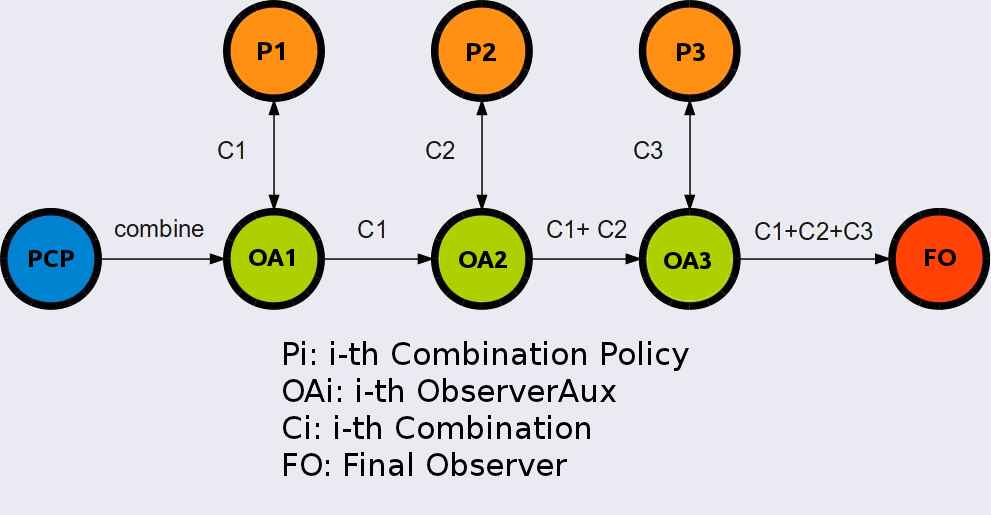
\includegraphics[scale=.23]{images/Comb2.jpg}
		\end{figure}
  \end{exampleblock}
}

\frame{
  \frametitle{Lado Com\'un}
  \begin{exampleblock}{Ejemplo de una pol\'itica compuesta}
    Supongamos un vestidor, con diferentes prendas de vestir.
		\begin{figure}[H]\hspace{.3cm}
			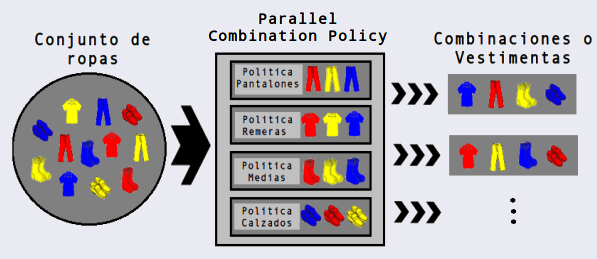
\includegraphics[scale=.45]{images/sequencial_ropa.png}
		\end{figure}
  \end{exampleblock}
}

\frame{
  \frametitle{Lado Com\'un}
    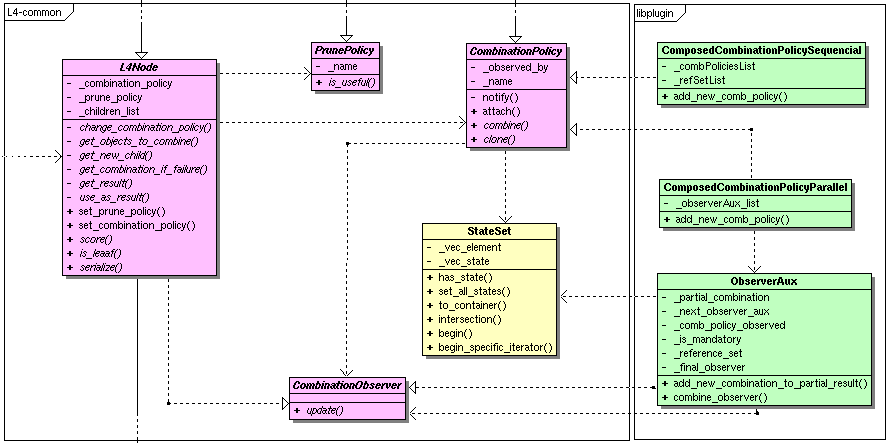
\includegraphics[scale=.35]{images/commonZoom.png}
}

\frame{
  \frametitle{Lado Com\'un}
  \textbf{El Nodo}\\
  Es un concepto abstracto de \textit{estado} de una aplicaci\'on implementada sobre \textbf{CombEng}.
		\begin{figure}[H]\hspace{.3cm}
			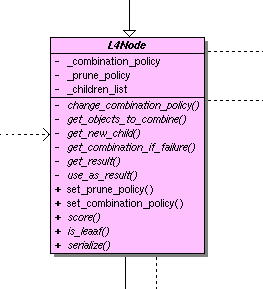
\includegraphics[scale=.5]{images/node.png}
		\end{figure}
}

\frame{
  \frametitle{Lado Com\'un}
    \begin{block}{Caracter\'isticas del nodo}
      \begin{description}
        \item[Es autosuficiente]: Encapsula la informaci\'on de inter\'es para la aplicaci\'on. Dispone del conocimiento necesario para procesar tal
          informaci\'on.
        \item[Es un observador]: el nodo es qui\'en observa a la pol\'itica de combinaci\'on.
        Por cada nueva combinaci\'on que la pol\'itica del nodo corriente genere, \'este ser\'a notificado y evaluar\'a, mediante su pol\'itica de poda,
        si dicha combinaci\'on es \'util. En caso afirmativo, crear\'a un nuevo nodo del nivel 5 (de ahora en m\'as lo llamaremos \texttt{L5Node}) y lo
        pondr\'a en su lista de hijos (\texttt{\_children\_list}). 
        \item[Es una unidad de trabajo]: establece el progreso general de la ejecuci\'on. Es decir, a partir de la informaci\'on que contiene, genera
          sus hijos inmediatos del \'arbol invocando al m\'etodo \texttt{call()}.
      \end{description}
    \end{block}
}

\frame{
\frametitle{El m\'etodo \texttt{call()}}
%  \textbf{El m\'etodo \texttt{call()}}
		\begin{figure}[H]\hspace{.3cm}
			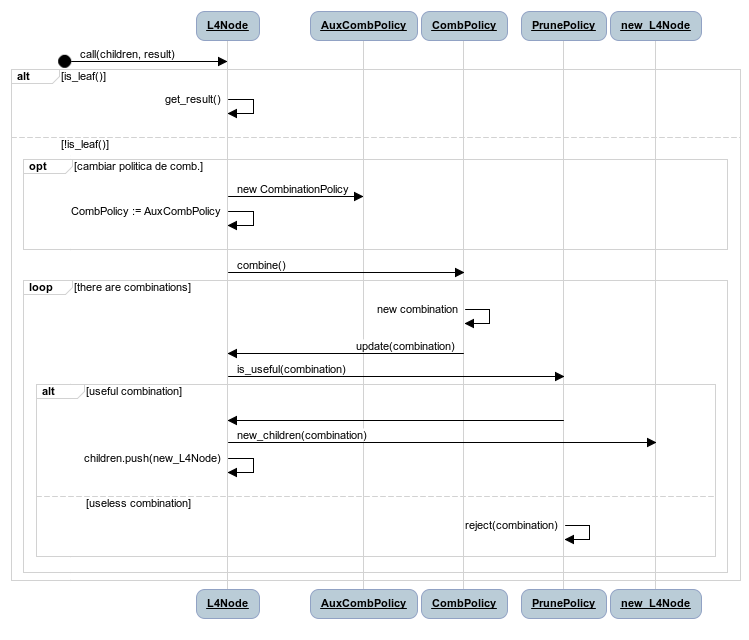
\includegraphics[scale=.33]{images/Call.png}
		\end{figure}
}

\subsection{Implementaci\'on}
\frame{
  \frametitle{?`C\'omo funciona una aplicaci\'on que usa \textbf{CombEng}?}
    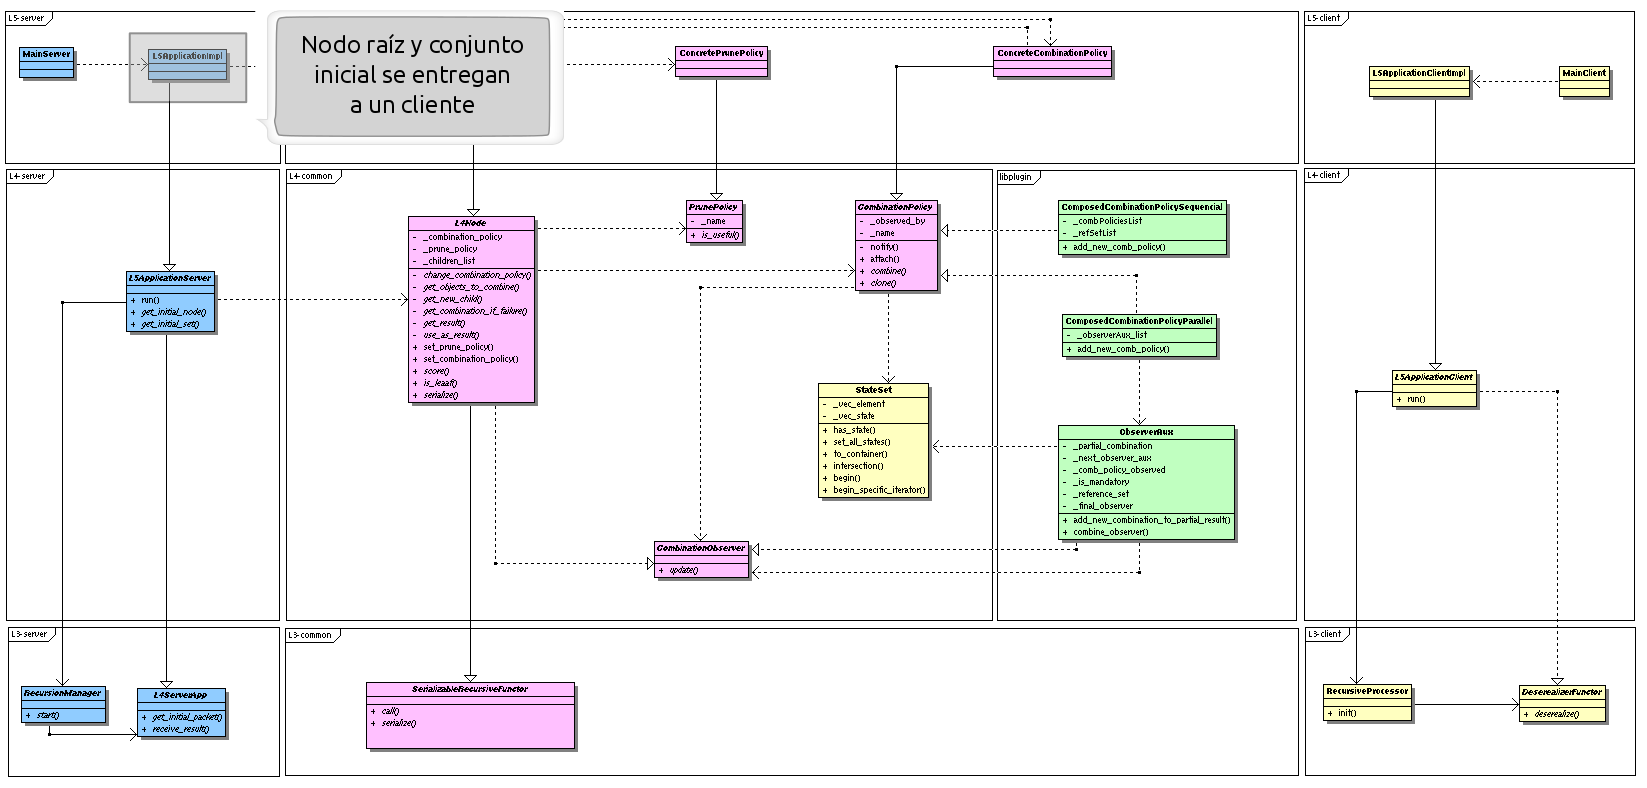
\includegraphics[scale=.2]{images/resumenServer.png}
  }

\frame{
  \frametitle{?`C\'omo funciona una aplicaci\'on que usa \textbf{CombEng}?}
    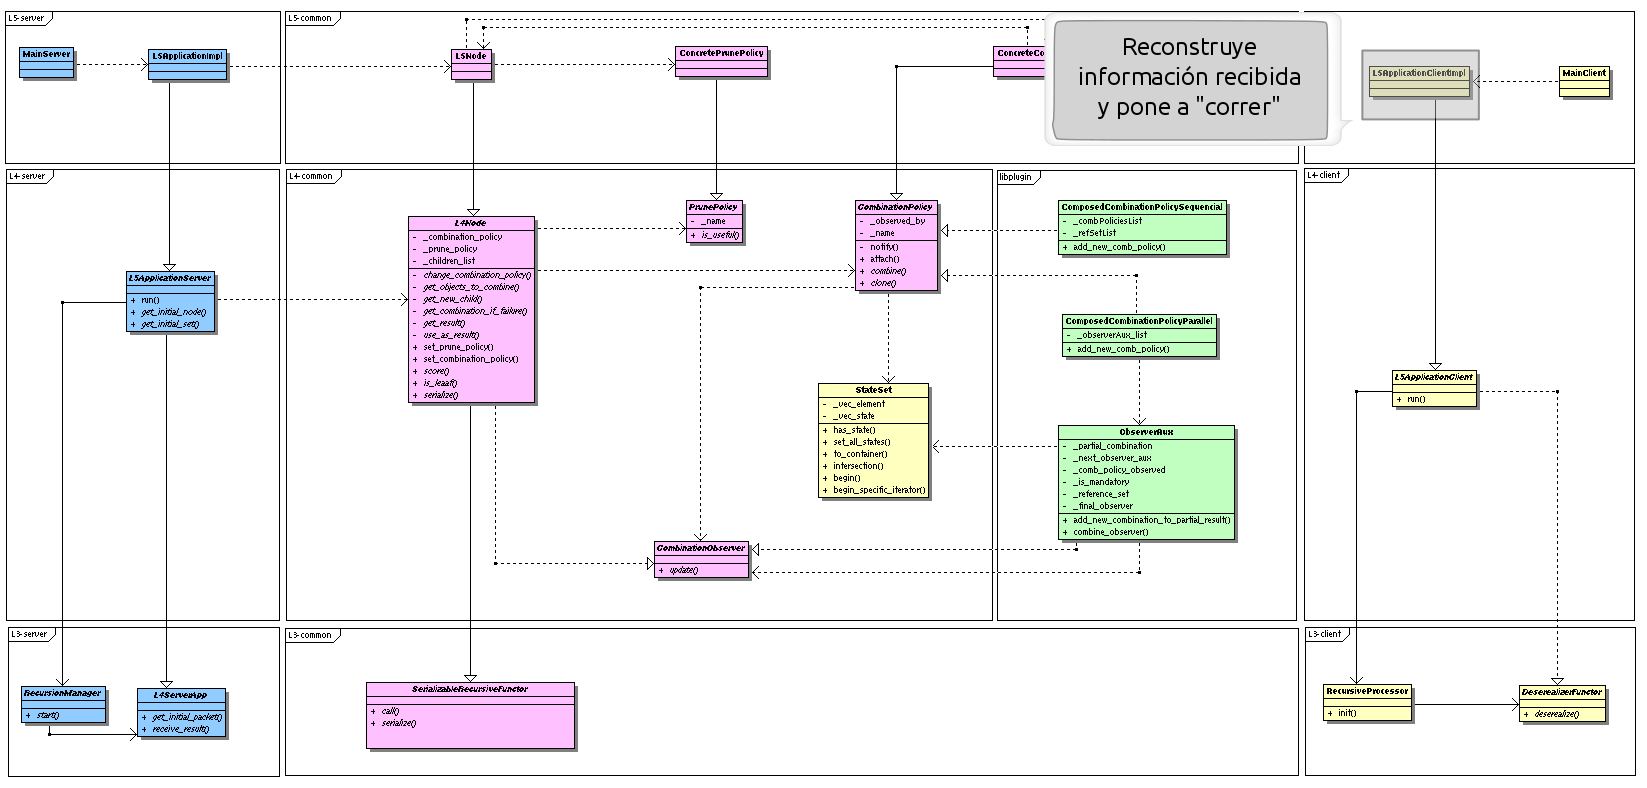
\includegraphics[scale=.2]{images/resumenClient.png}
  }

\frame{
  \frametitle{?`C\'omo funciona una aplicaci\'on que usa \textbf{CombEng}?}
    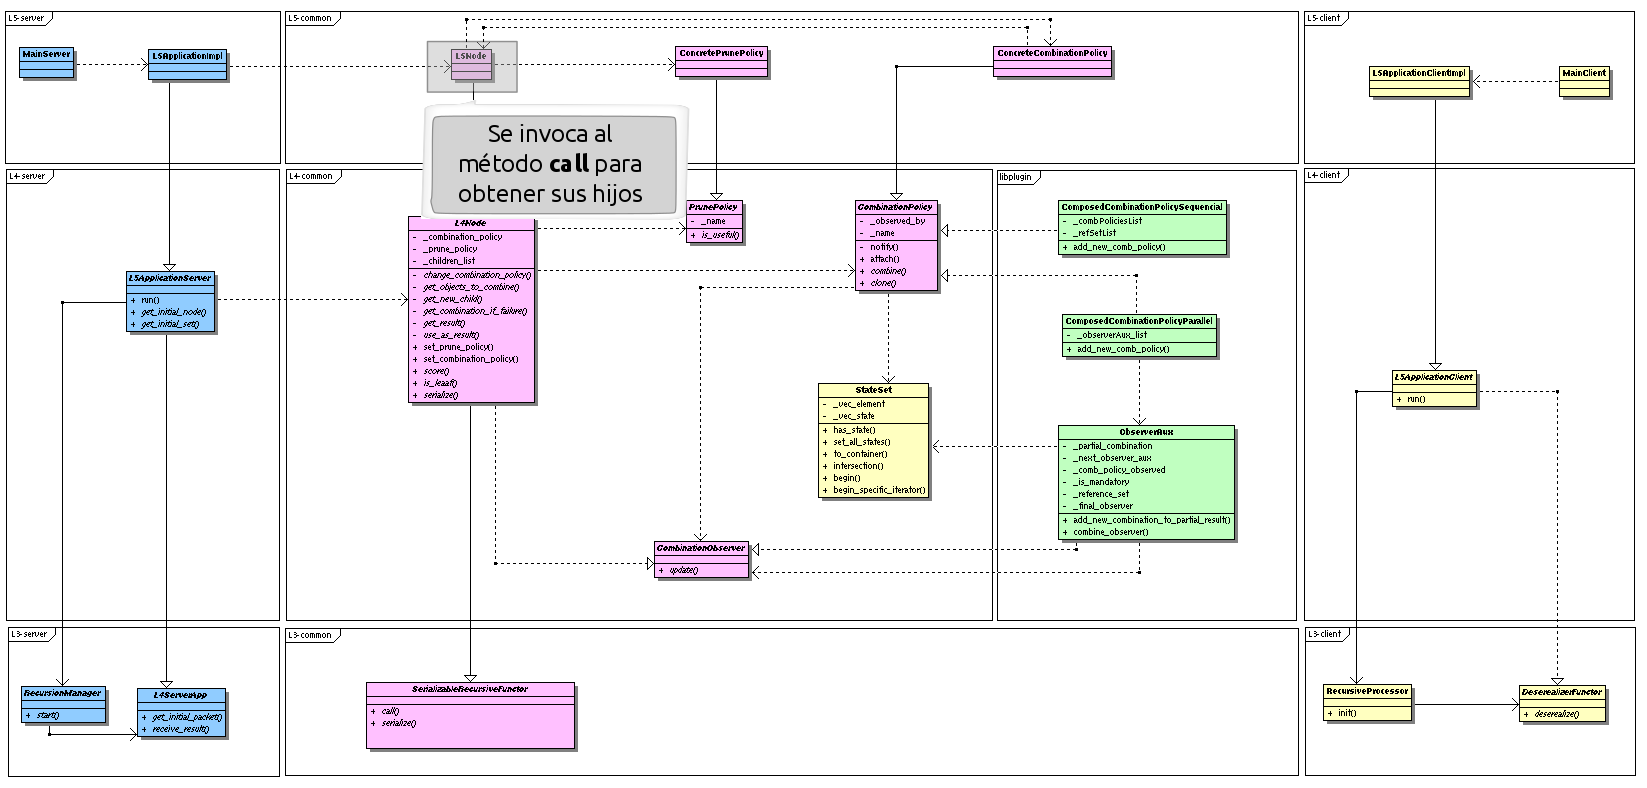
\includegraphics[scale=.2]{images/resumenNode.png}
  }

\frame{
  \frametitle{?`C\'omo funciona una aplicaci\'on que usa \textbf{CombEng}?}
    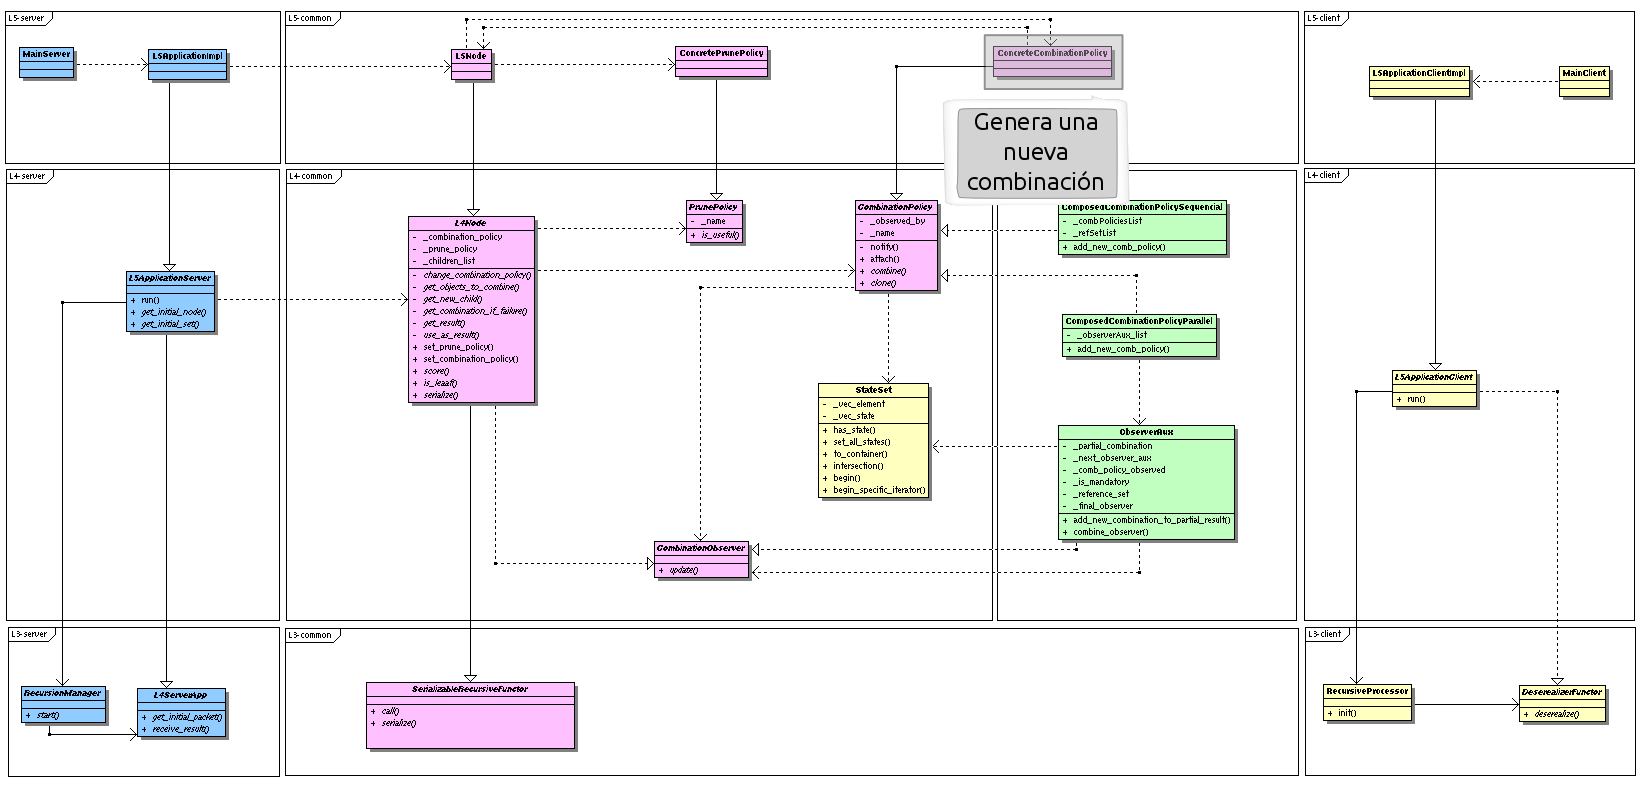
\includegraphics[scale=.2]{images/resumenCombPolicy.png}
  }

\frame{
  \frametitle{?`C\'omo funciona una aplicaci\'on que usa \textbf{CombEng}?}
    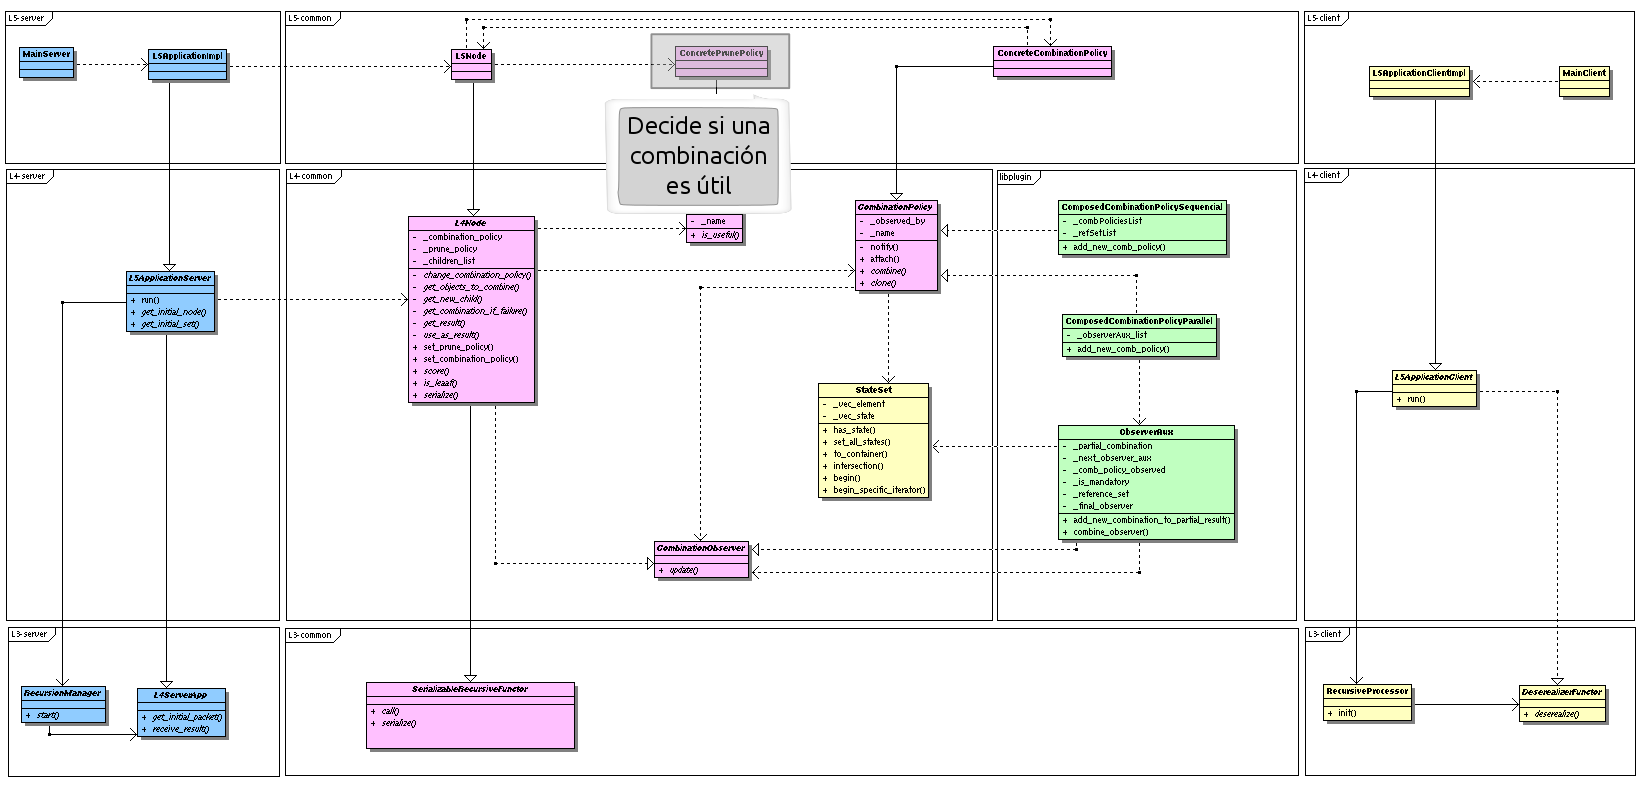
\includegraphics[scale=.2]{images/resumenPrunePolicy.png}
  }

\frame{
  \frametitle{?`C\'omo funciona una aplicaci\'on que usa \textbf{CombEng}?}
    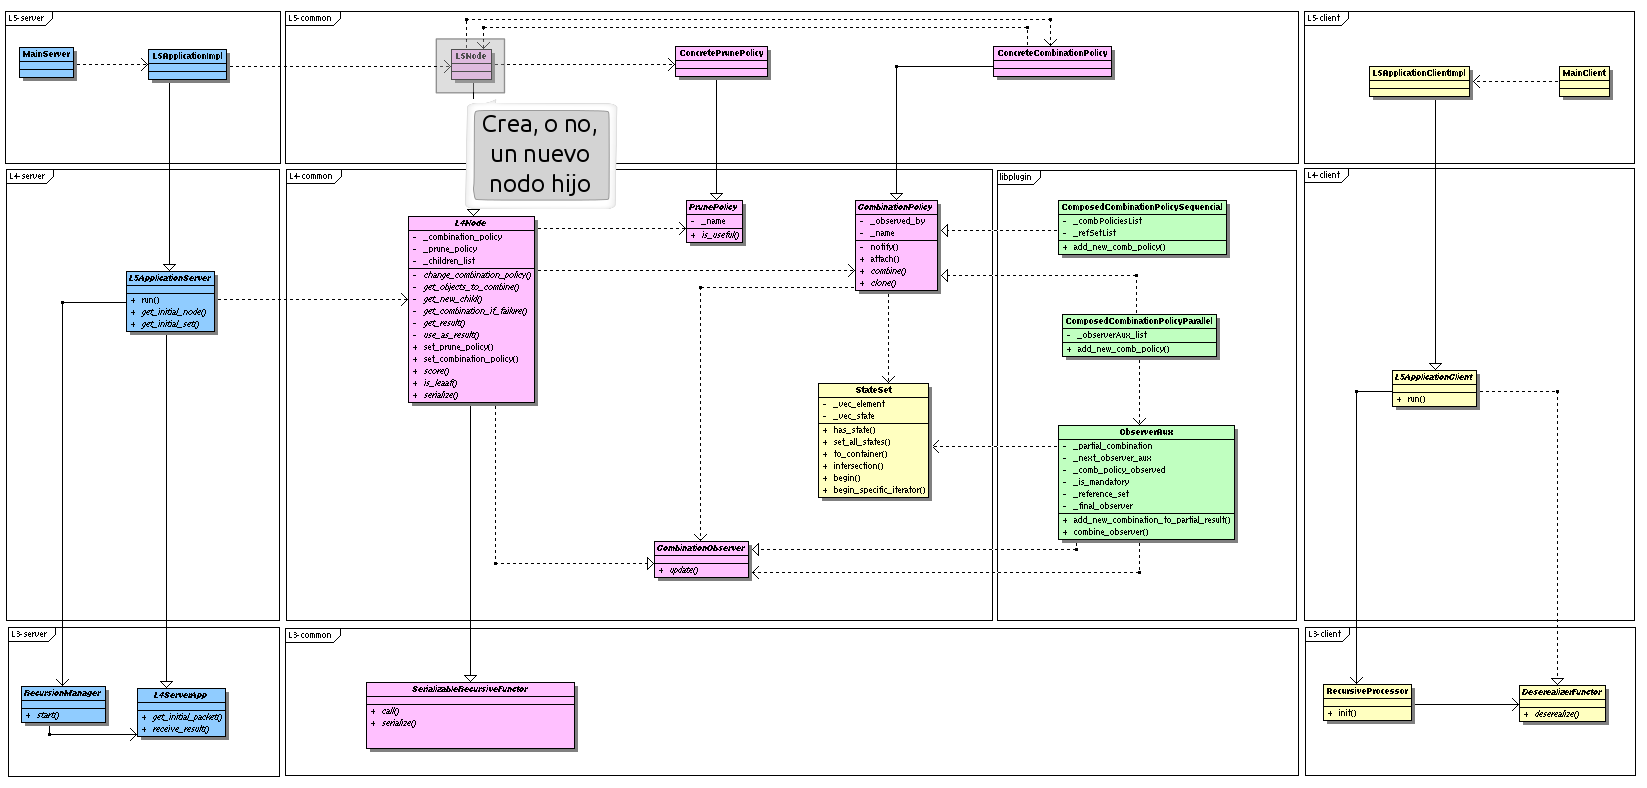
\includegraphics[scale=.2]{images/resumenNode2.png}
  }

\frame{
\frametitle{?`C\'omo funciona una aplicaci\'on que usa \textbf{CombEng}?}
Para hacer uso del framework, el desarrollador de una nueva aplicaci\'on deber\'a implementar aquellas interfaces definidas por \textbf{CombEng}.
\begin{block}{Por el lado \textbf{servidor}}
  \begin{figure}[h]
    \begin{minipage}{3.3cm}
      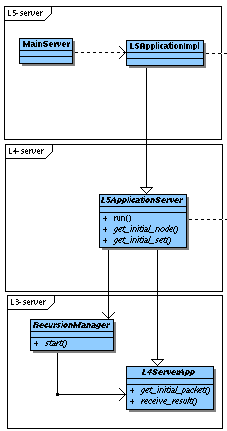
\includegraphics[scale=.35]{images/server.png}
    \end{minipage}
    \begin{minipage}{0.67 \textwidth} % 0.5 \textwidth = 50% ancho de página
      \begin{itemize}
		  \item \texttt {get\_initial\_packet}: Retorna un paquete de datos representando al nodo inicial de la aplicaci\'on. Dicho nodo es enviado a
        un cliente, para que sea \'el quien inicie la ejecuci\'on de la aplicaci\'on.
		  \item \texttt {receive\_result}: Durante el procesamiento de un nodo, los clientes pueden enviar resultados al servidor. Este m\'etodo es quien
        decide qu\'e hacer con los mismos.
        \end{itemize}
      \end{minipage}
    \end{figure}
  \end{block}
}

\frame{
\frametitle{?`C\'omo funciona una aplicaci\'on que usa \textbf{CombEng}?}
\begin{block}{Por el lado \textbf{cliente}}
  \begin{figure}[h]
    \begin{minipage}{4cm}
      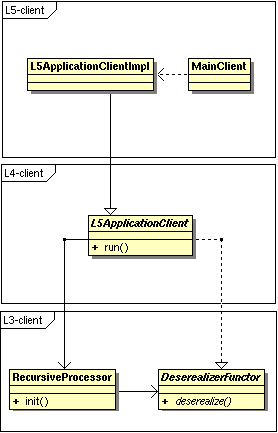
\includegraphics[scale=.35]{images/client.png}
    \end{minipage}
    \begin{minipage}{0.6 \textwidth} % 0.5 \textwidth = 50% ancho de página
      \begin{itemize}
        \item \texttt {deserialize}: Este m\'etodo efect\'ua el proceso de conversi\'on de un paquete que viaja por la red (\emph {binary-stream}) a un nodo
        utilizable por la aplicaci\'on. 
      \end{itemize}
      \end{minipage}
    \end{figure}
  \end{block}
}

 \frame{
 \frametitle{?`C\'omo funciona una aplicaci\'on que usa \textbf{CombEng}?}
 \begin{block}{Por el lado en com\'un}
   \begin{minipage}{3.3cm}
     \begin{center}
       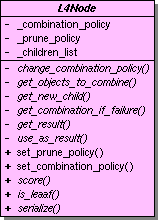
\includegraphics[scale=.43]{images/node-blue.png}
     \end{center}
   \end{minipage}
   \begin{minipage}{0.67 \textwidth} % 0.5 \textwidth = 50% ancho de página
     \begin{itemize}
         \footnotesize{} \vspace{.5cm}
       \item \texttt{void serialize(recabs::Packet\& pkt)}
       \item \texttt{void get\_objects\_to\_combine(std::list<T>\&)}
       \item \texttt{float score()}
       \item \texttt{bool use\_as\_result()}
       \item \texttt{recabs::Packet get\_result()}
       \item \texttt{bool is\_leaf()}
     \end{itemize}
   \end{minipage}
   \begin{itemize}
     \footnotesize{}
     \item \texttt{CombinationPolicy<T>* change\_combination\_policy()}
     \item \texttt{void new\_children(const std::list<T>\&  combination, std::list<L4Node*>\&)}
     \item \texttt{CombinationPolicy<T>* get\_combination\_if\_failure(const std::string\& failed\_comb\_policy)}
   \end{itemize}
 \end{block}
 }

%COMO PRIMER PASO, breve introduccion de lo que consiste el trabajo, a quienes involucra, etc.
\section{Aplicaci\'on RNA Folding Free Energy}
\subsection{Motivaci\'on y Problema}
\frame{
    \frametitle{Introducci\'on al VIH}
    \begin{block}{El Virus VIH}
      El \textit{Virus de Inmunodeficiencia Humana} no puede reproducirse por s\'i mismo, sino que precisa de la maquinaria celular para lograrlo.
      Infecta a c\'elulas de un organismo vivo para duplicarse.
    \end{block}
    \pause
    \begin{block}{El Sistema Inmunol\'ogico}
      Es el encargado de eliminar las infecciones que pueden ingresar en el organismo. El VIH ataca al sistema inmunol\'ogico mismo, aquel
      encargado de eliminarlo.
    \end{block}
    \pause
    \begin{block}{El SIDA}
      El \textit{S\'indrome de Inmunodeficiencia Adquirida} es un cuadro cl\'inico. A una persona infectada por el virus VIH se le diagnostica
      SIDA cuando su sistema inmunol\'ogico es demasiado d\'ebil para combatir las infecciones.
    \end{block}
}

% \frame{
%     \frametitle{Tratamientos}
%     \begin{block}{Monoterapia}
%       En 1987, se aprob\'o el uso de la \textit{zidovudine} en la prevenci\'on de la replicaci\'on del VIH.
%       \vspace{-.41cm}
%      \begin{center}
%         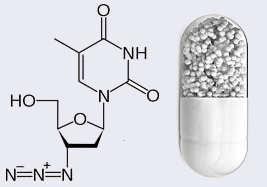
\includegraphics[scale=.2]{images/zidovudine.png}
%       \end{center}
%     \end{block}
%     \pause
%     \begin{block}{HAART}
%         En 1996, se reemplaza la monoterapia por el \textit{Tratamiento Antirretroviral de Gran Actividad} (del ingl\'es HAART).
%         %la expansi\'on en la s\'intesis de diferentes clases de antirretrovirales hizo posible reemplazar la monoterapia por el
%     \end{block}
%     \pause
%     \begin{block}{Adherencia al Tratamiento}
%         \begin{itemize}
%             \item Una buena adherencia contribuye a evitar la resistencia a los f\'armacos.
%               \pause
%             \item Caso contrario, se da lugar a la aparici\'on de mutantes del VIH no susceptibles a los efectos de la medicaci\'on.
%         \end{itemize}
%     \end{block}
% }

\frame{
    \frametitle{El Interrogante}
    Cuando a una persona infectada con VIH se le aplica un antirretroviral, el virus comienza a mutar hasta que logra hacerse resistente. El orden en que se aplican los antirretrovirales y c\'omo \'estos son combinados, son factores muy importantes que determinan, o entre otras cosas, el tiempo que transcurrir\'a hasta el momento en que el virus sea resistente a todos los antirretrovirales.

    \vspace{0.3cm} 
    \pause
    \begin{block}{Interrogante}
        \textit{?`Tiene alg\'un impacto el suministro de antirretrovirales sobre la estructura secundaria de las mutantes resultantes?}
    \end{block}
}

\subsection{Marco Te\'orico}
\frame{
    \frametitle{Organismos y Mol\'eculas}
    \begin{block}{Organismo}
      Conjunto de biomol\'eculas org\'anicas e inorg\'anicas organizadas de manera especifica para cumplir determinadas funciones e interactuar con el medio en que se encuentran.
    \end{block}

    \begin{block}{Nucle\'otidos}
      Peque\~nas mol\'eculas org\'anicas constituyentes de macromol\'eculas de mayor complejidad. Los 5 tipos de nucle\'otidos m\'as importantes son:
	    \begin{enumerate}
	      \item Adenina (A) compone el ADN y el ARN.
	      \item Guanina (G) compone el ADN y el ARN.
	      \item Timina (T) compone el ADN.
	      \item Citosina (C) compone el ADN y el ARN.
	      \item Uracilo (U) compone el ARN.
	    \end{enumerate}
    \end{block}
}
  
\frame{
  \frametitle{Organismos y Mol\'eculas}
    \begin{block}{Amino\'acidos}
      Son mol\'eculas que conforman las prote\'inas y son esenciales para la vida. A continuaci\'on se muestra una tabla conteniendo algunos amino\'acidos y sus abreviaciones.
      \begin{center}
        \begin{tabular}{|ccc|}
          \hline Nombre & Ab. 3 letras & Ab. 1 Letra \\ 
          \hline Alanine & Ala & A \\ 
          \hline Arginine & Arg & R \\ 
          \hline Asparagine & Asn & N \\ 
          \hline Aspartic acid & Asp & D \\ 
          \hline Cytesine & Cys & C \\ 
          \hline Glutamic acid & Glu & E \\ 
          \hline Glutamine & Gln & Q \\ 
          \hline Glycine & Gly & G \\ 
          \hline   ... &  ...  & ... \\ 
          \hline 
        \end{tabular} 
      \end{center}

    \end{block}
}

 \frame{
 \frametitle{Organismos y Mol\'eculas}
 
 \begin{block}{\'Acidos Nucleicos}
    Son grandes mol\'eculas que codifican toda la informaci\'on necesaria para la vida. Las mismas, est\'an conformadas por secuencias de nucle\'otidos espec\'ificas. La informaci\'on gen\'etica est\'a codificada mediante sucesivos codones (tripletes de nucle\'otidos que codifican un amino\'acido).
       Existen dos tipos de \'Acidos nucleicos:
       \begin{itemize}
	  \item \textbf{ADN}: Est\'a formado por desoxi-ribonucle\'otidos \emph{(\'acido desoxi-ribonucleico)}.
	  \item \textbf{ARN}: Est\'a formado por ribonucle\'otidos \emph{(\'acido ribonucleico)}.
       \end{itemize}
       Ambos, comparten ciertas cualidades:
	\begin{enumerate}
	  \item Pueden estar compuestos por una hebra simple o doble de nucle\'otidos.
	  \item Se heredan de generaci\'on en generaci\'on.
	  \item Cifrar la informac\'on gen\'etica.
	\end{enumerate}
 \end{block}
 }

\frame{
\frametitle{Organismos y Mol\'eculas}
  \begin{block}{Ejemplo de \'acidos nucleicos}
    \begin{center}
      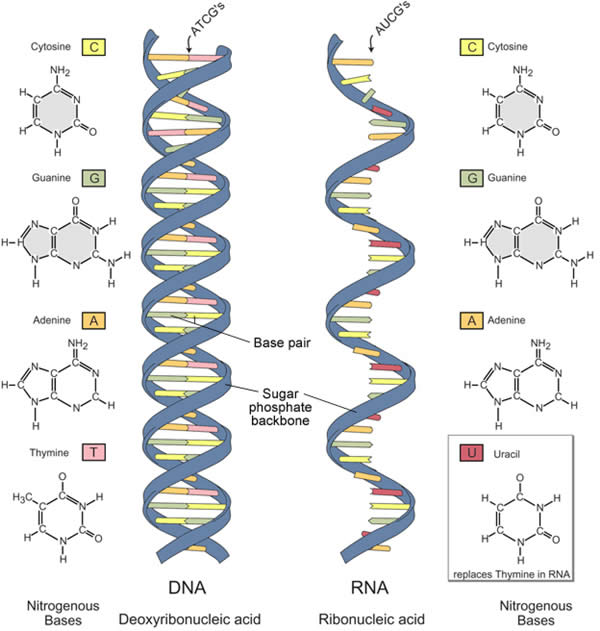
\includegraphics[scale=0.25]{images/dna_rna.png}
    \end{center}
  \end{block}
}


\frame{
  \frametitle {\'Acidos Nucleicos}     
    \begin{block}{ARN}
	\begin{figure}[h]
	  \begin{minipage}{0.7 \textwidth} % 0.5 \textwidth = 50% ancho de página
	    Generalmente, consiste en una hebra de cadena simple, la cual usualmente es trascripta a partir de una porci\'on de ADN y se utiliza posteriormente en la c\'elula para la s\'intesis de prote\'inas. Algunos virus poseen ARN como \'unico material gen\'etico cuya monohebra puede plegarse, dando lugar a lo que se conoce como estructura secundaria.
	  \end{minipage}
	  \begin{minipage}{3cm}% También se puede indicar en cms
	    \begin{center}
	      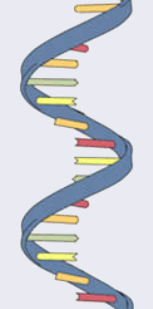
\includegraphics[scale=.3]{images/arn.png}
	    \end{center}
	  \end{minipage}
	\end{figure}
    \end{block}

    \begin{block}{La Estructura Primaria y Secundaria Del ARN}
	La estructura primaria del ARN, es una secuencia de nucle\'otidos de longitud $n$, $A=a_{1}a_{2}a_{3}\dots a_{n}$ con $a_{i} \in \left\lbrace A, U, G, C \right\rbrace$. El plegamiento de una secuencia de ARN entre sus bases complementarias determina lo que se denomina estructura secundaria de ARN.

    \end{block}
}


\frame{
  \frametitle {Energ\'ia libre y Estabilidad}     
  El concepto de ``Energ\'ia Libre'' hace referencia a la energ\'ia total contenida en un sistema, la cual le permite al mismo realizar determinados  trabajos, por ejemplo, una mol\'ecula de ARN con estructura secundaria, puede usar su energ\'ia libre para plegarse hacia una estructura secundaria m\'as estable. De este modo, un ARN con una estructura secundaria estable, implica una mol\'ecula en la cual sus interacciones el\'ectricas entre nucle\'otidos se hallan completamente neutralizadas. Se podr\'ia inferir que si una secuencia viral de ARN mutada tiene energ\'ia libre m\'inima, la misma no variar\'a su estructura secundaria por s\'i sola. 
}


\frame{
  \frametitle {El virus VIH}
    Los virus son entidades infecciosas microsc\'opicas que pueden multiplicarse dentro de las c\'elulas de un organismo dado. El virus VIH
    infecta a c\'elulas vitales como:
      \begin{itemize}
       \item \textit{Linfocitos T} (espec\'ificamente los que contienen receptores CD4)
       \item \textit{Macr\'ofagos} 
       \item \textit{C\'elulas dendr\'iticas}
      \end{itemize}
    Las CD4$^+$ son un sub-grupo de los linfocitos, un tipo de gl\'obulos blancos, los cuales desempe\~nan un rol importante en el establecimiento y maximizaci\'on del sistema de defensa de un organismo.
}



\frame{
  \frametitle {Antirretrovirales}
  Los f\'armacos utilizados en tratamientos actuales para combatir las infecciones con VIH son denominados antirretrovirales. Existe una variedad de estos provenientes de distintos laboratorios, cada uno con sus respectivas caracter\'isticas, los cuales se clasifican por su rango de acci\'on en varias clases: 
    \begin{itemize}
      \item \emph{Protease Inhibitors} (PI)
      \item \emph{Reverse Transcriptase Inhibitors}
	  \begin{enumerate}
	    \item \emph{Nucleotide Reverse Transcriptase Inhibitors} (NRTI)
	    \item \emph{Non-Nucleotide Reverse Transcriptase Inhibitors} (NNRTI)
	  \end{enumerate}
      \item \emph{Fusion or Entry Inhibitors}
      \item \emph{Integrase Inhibitors}
  \end{itemize}
   El objetivo de aplicar antirretrovirales a los pacientes es inhibir la replicaci\'on del virus por un tiempo indeterminado. 
}


% \frame{
%   \frametitle {Antirretrovirales}
%     \begin{block} {Terapia antirretroviral de Gran Actividad}
%       Este tipo de terapia consiste en la administraci\'on simult\'anea de distintos antirretrovirales pertenecientes a diferentes grupos.
% 
%     \end{block}
% 
%     \begin{block} {Fallo virol\'ogico}
%      Aunque el paciente est\'e tomando los medicamentos, la cantidad de virus en sangre no disminuye o bien se eleva repetidamente.
%     \end{block}
% 
%     \begin{block}{Fallo inmunol\'ogico}
%       Aunque el paciente tome los medicamentos, el recuento de linfocitos CD4+ no disminuye ni se incrementa.     
%     \end{block}
% 
%     \begin{block}{Fallo cl\'inico}
%       Aunque el paciente toma los medicamentos antirretrovirales, persisten los s\'intomas de infecci\'on por VIH.     
%     \end{block}
% }


\subsection{Soluci\'on}
\frame{
    \frametitle{Retomando el Problema...}
    \begin{block}{}
        \textit{?`Tiene alg\'un impacto el suministro de antirretrovirales sobre la estructura secundaria de las mutantes resultantes?}
    \end{block}
    \vspace{.1cm} 
    \textbf{Propuesta de Soluci\'on:}
    \begin{block}{}
      %Se intenta dar un abordaje inicial a lo formulado anteriormente, mediante el 
      Desarrollo de una aplicaci\'on de software que, recibiendo como entrada una \textit{secuencia inicial del virus} y los \textit{antirretrovirales}
      disponibles hasta el momento, permita analizar c\'omo las diferentes terapias pueden afectar, o no, a la \textbf{estructura secundaria} y si esta
      posible afecci\'on puede ser un factor en la evoluci\'on viral. 
      La soluci\'on consta de:
      \begin{enumerate}
	\item La generaci\'on de un \'arbol, donde cada rama representar\'a una terapia y la variaci\'on de la FE a medida que se avanza en la misma.
	\item El an\'alisis de cada uno de los camino del \'arbol.
      \end{enumerate}   
    \end{block}
}

\frame{

    \frametitle{Soluci\'on}
    \begin{block}{Generaci\'on del \'arbol}
      \begin{enumerate}
      \item Tomar una secuencia en representaci\'on del virus y todos los antirretrovirales conocidos hasta el momento.
      \pause
      \item Seleccionar los antirretrovirales que realmente pueden ser aplicados a la secuencia. De no haber ninguno aplicable, saltar al paso 7.
      \pause
      \item Combinar los antirretrovirales seleccionados en el paso anterior.
      \pause
      \item Aplicar cada combinaci\'on a la secuencia y obtener las secuencias mutantes.
      \pause
      \item Calcular la FE de cada mutante.
      \pause
      \item Ejecutar este proceso para cada una de las mutantes obtenidas, luego, saltar al paso 8.
      \pause
      \item Informar resultado.
      \item Terminar.
      \end{enumerate}
    \end{block}
}

\frame{
    \begin {block} {}
      \frametitle{Soluci\'on}
      \begin{center}
	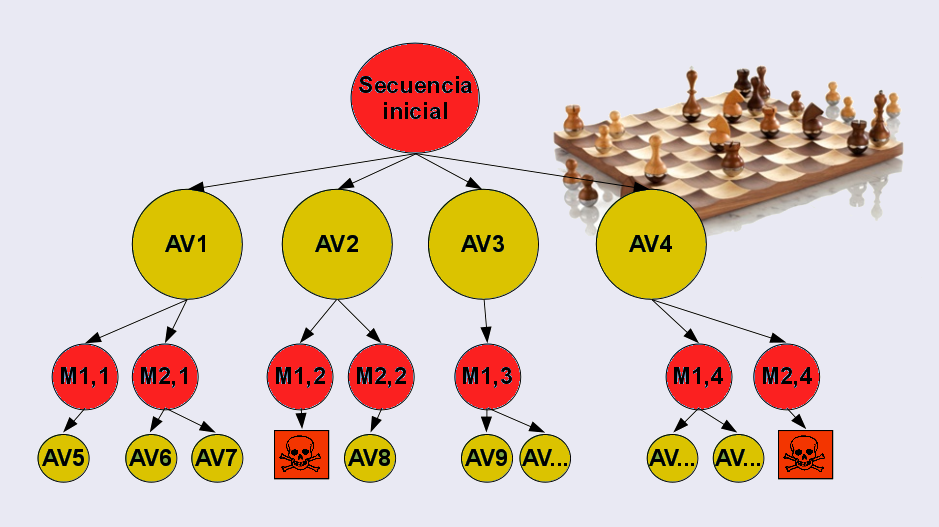
\includegraphics[width=\linewidth]{images/Arbol_ajedrez.png}
      \end{center}
    \end{block}
}

\frame{
    \frametitle{Implementaci\'on}
    
    \begin{block}{}
      Como vimos anteriormente, la soluci\'on consta de armar un \'arbol y analizar los distintos caminos del mismo. Se decidi\'o usar \textbf{FuD} por las siguientes razones:
      \begin{itemize}
	\item El c\'alculo de la energ\'ia libre requiere un gran costo computacional.
	\item El \'arbol contendr\'a una gran cantidad de nodos.
	\item La necesidad de contar con un motor combinatorio para combinar antirretrovirales.
      \end{itemize}

      Esto nos brinda dos ventajas imprescindibles:
	\begin{enumerate}
	  \item La posibilidad de poder realizar los c\'omputos de manera distribuida.
	  \item Realizar, eficientemente, las combinaciones de antirretrovirales usando distintas pol\'iticas de combinaci\'on.
	\end{enumerate}
    \end{block}
}


\frame{

    \frametitle{Soluci\'on}
    \begin{block}{Generaci\'on del \'arbol}
      \begin{enumerate}
      \item \textbf {Tomar una secuencia en representaci\'on del virus y todos los antirretrovirales conocidos hasta el momento.}
      \item \textbf Seleccionar los antirretrovirales que realmente pueden ser aplicados a la secuencia. De no haber ninguno aplicable, saltar al paso 7.
      \item Combinar los antirretrovirales seleccionados en el paso anterior.
      \item Aplicar cada combinaci\'on a la secuencia y obtener las secuencias mutantes.
      \item Calcular la FE de cada mutante.
      \item Ejecutar este proceso para cada una de las mutantes obtenidas, luego, saltar al paso 8.
      \item Informar resultado.
      \item Terminar.
      \end{enumerate}
    \end{block}
}



\begin{frame}[fragile]
    \frametitle{Implementaci\'on - Datos de entrada}
    La aplicaci\'on recibe dos entradas:
    \begin{block}{Secuencia inicial del virus}
	Archivo que contiene una secuencia de nucle\'otidos (ADN del virus).
	\scriptsize
       \begin{lstlisting}[basicstyle=\tt, frame=trBL, tabsize=4,fontadjust=true]
	  CCTCAGGTCACTCTTTGGCAACGACCCCTGATAGGGGGGCAACTAAAGGAAGCCAGG...
	\end{lstlisting}
    \end{block}
    \normalsize
    \begin{block}{Conjunto de antirretrovirales}
      Archivo .xml conteniendo la base de datos de antirretrovirales.
      \scriptsize
	\begin{lstlisting}[basicstyle=\tt, frame=trBL, tabsize=4] 
	<antivirals>
	   <antiviral id="Didanosine" num ="1" type ="tRT" class ="cNRTI">	
	       <resistance pos="164" aminos="R"/>
	       <resistance pos="173" aminos="V"/>
	    </antiviral>
	    ...
	</antivirals>
	\end{lstlisting}
	\normalsize
    \end{block}
\end{frame}


% \frame{
%     \frametitle{Implementaci\'on - Representaci\'on de datos}
%     \begin{block}{Secuencia de Nucle\'otidos}
%       Se utilizan expresiones regulares para representar las estructuras:
%       \begin{itemize}
% 	\item $nuc\_arn = a \vert u \vert c \vert g \vert \_$
% 	\item $nuc\_adn = a \vert t \vert c \vert g \vert \_$ 
% 	\item $gen\_arn = (nuc\_arn)^{+}$
% 	\item $gen\_adn = (nuc\_adn)^{+}$	
%       \end{itemize}
%     \end{block}
% 
%     \begin{block}{Antirretrovirales}
%       Un Antirretroviral consta, principalmente, de un listado de pares $<pos , aminos>$, donde $pos \geq 0$ y $aminos$ es una lista de amino\'acidos. 
% 	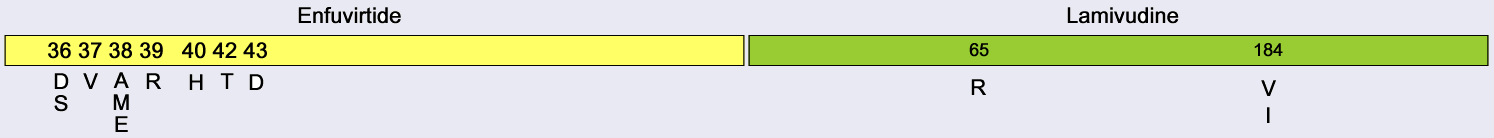
\includegraphics[scale=.4]{images/Antivirals.png}\\
%       Adem\'as, se incluye otro tipo de informaci\'on para el antirretroviral, como un identificador, un nombre, una clase y un tipo.
%     \end{block}
% }


\frame{

    \frametitle{Soluci\'on}
    \begin{block}{Generaci\'on del \'arbol}
      \begin{enumerate}
      \item \textbf {Tomar una secuencia en representaci\'on del virus y todos los antirretrovirales conocidos hasta el momento.}
      \item \textbf {Seleccionar los antirretrovirales que realmente pueden ser aplicados a la secuencia. De no haber ninguno aplicable, saltar al paso 7.}
      \item Combinar los antirretrovirales seleccionados en el paso anterior.
      \item Aplicar cada combinaci\'on a la secuencia y obtener las secuencias mutantes.
      \item Calcular la FE de cada mutante.
      \item Ejecutar este proceso para cada una de las mutantes obtenidas, luego, saltar al paso 8.
      \item Informar resultado.
      \item Terminar.
      \end{enumerate}
    \end{block}
}



\frame{
    \frametitle{Implementaci\'on - Selecci\'on de antirretrovirales}
    En una primera instancia, se seleccionan aquellos a los que el virus no es resistente, luego se elijen aquellos que representan mas obst\'aculos para el virus.
    \begin{block}{Resistencia a un antirretroviral}
      Un antirretroviral esta compuesto, entre otras cosas, por un conjunto de resistencias. Tomemos el antirretroviral Abacavir.
      \vspace{-0.2cm}
      \begin{figure}[H]
	
\includegraphics[width=\linewidth]{images/abacadir.png}
      \end{figure}
      \vspace{-0.4cm}
      Luego, si el triplete n\'umero \textbf{65} de la secuencia codifica el amino\'acido \textbf{R}, significa que dicha secuencia es resistente a tal antiviral.
      \vspace{-0.4cm}
      \begin{figure}[H]
	
\includegraphics[width=\linewidth]{images/secuencia.png}
      \end{figure}
      \vspace{-0.4cm}
      En este caso, el triplete \textbf{ATT} codifica el amino\'acido \textbf{R}, lo cual hace a la mutante resistente al antirretroviral Abacavir.\\
    \end{block}
    
}

\frame{
    \frametitle{Soluci\'on}
    \begin{block}{Generaci\'on del \'arbol}
      \begin{enumerate}
      \item \textbf {Tomar una secuencia en representaci\'on del virus y todos los antirretrovirales conocidos hasta el momento.}
      \item \textbf {Seleccionar los antirretrovirales que realmente pueden ser aplicados a la secuencia. De no haber ninguno aplicable, saltar al paso 7.}
      \item \textbf {Combinar los antirretrovirales seleccionados en el paso anterior.}
      \item Aplicar cada combinaci\'on a la secuencia y obtener las secuencias mutantes.
      \item Calcular la FE de cada mutante.
      \item Ejecutar este proceso para cada una de las mutantes obtenidas, luego, saltar al paso 8.
      \item Informar resultado.
      \item Terminar.
      \end{enumerate}
    \end{block}
}


\frame{
    \frametitle{Implementaci\'on - Combinaci\'on de antirretrovirales}

    \begin{block}{?`Por qu\'e combinar antirretrovirales?}
	Los antirretrovirales individualmente no suprimen la infecci\'on por VIH a largo plazo, por lo cual, actualmente se usan combinaciones de \'estos. Las combinaciones de antirretrovirales act\'uan incrementando el n\'umero de obst\'aculos para la mutaci\'on viral, manteniendo bajo el n\'umero de copias virales. 
    \end{block}

    \begin{block}{?`C\'omo combinar los antirretrovirales?}
	Como se explic\'o anteriormente hay tres tipos de antirretrovirales (\textbf{NRTI}, \textbf{NNRTI}, \textbf{PI}), dependiendo de la cantidad de cada uno que pueden ser aplicados a la secuencia del nodo corriente, se escoge una pol\'itica de combinaci\'on.
	A continuaci\'on se muestra una M\'aquina de Estados Finita representando c\'omo los antirretrovirales son combinados
    \end{block}

}

\frame{
    \frametitle{Implementaci\'on - Combinaci\'on de antirretrovirales}
    \begin{block}{FSM para la combinaci\'on de antirretrovirales}
	\begin{figure}[ht]
	  \centering
	  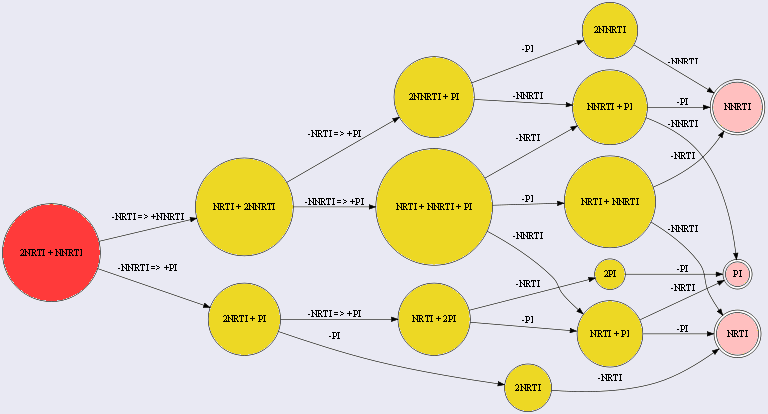
\includegraphics[width=\linewidth]{images/Antivirals_fsm.png}
	  \label{antivirals_fsm}
	\end{figure}
    \end{block}
}

\frame{
    \frametitle{Soluci\'on}
    \begin{block}{Generaci\'on del \'arbol}
      \begin{enumerate}
      \item \textbf {Tomar una secuencia en representaci\'on del virus y todos los antirretrovirales conocidos hasta el momento.}
      \item \textbf {Seleccionar los antirretrovirales que realmente pueden ser aplicados a la secuencia. De no haber ninguno aplicable, saltar al paso 7.}
      \item \textbf {Combinar los antirretrovirales seleccionados en el paso anterior.}
      \item \textbf{Aplicar cada combinaci\'on a la secuencia y obtener las secuencias mutantes.}
      \item Calcular la FE de cada mutante.
      \item Ejecutar este proceso para cada una de las mutantes obtenidas, luego, saltar al paso 8.
      \item Informar resultado.
      \item Terminar.
      \end{enumerate}
    \end{block}
}



\frame{
    \frametitle{Implementaci\'on - Generaci\'on de mutantes}
      Para lo obtenci\'on de las mutantes a partir de un conjunto de antirretrovirales, se desarroll\'o un algoritmo que puede ser resumido en los siguientes pasos:
    \begin{block}{1er paso}
        Obtener el producto cartesiano de las resistencias de cada antirretroviral. Suponga el siguiente ejemplo:\\
	\vspace{.4cm}
	\textbf{Antirretrovirales}:
	\vspace{-.85cm}
	\begin{center}
	  \emph {A = \{(1,G), (2,T)\}}
	
	  \emph {B = \{(3,G), (2,T), (4,R)\}}
	\end{center}
	En un par \emph{(X, Y)}: \emph{X} representa la posici\'on de la resistencia e \emph{Y} el amino\'acido al cual es resistente.\\
	\vspace{0.2cm}
	Luego, el producto cartesiano entre \emph{A} y \emph{B} es:\\
	%\vspace{.1cm}
	\textbf{\emph{A} x \emph{B    =}} \vspace{-.65cm}
	\begin{center}
	  \emph{\{\{(1,G), (3,G)\}, \{(1,G), (2,T)\}, \{(1,G), (4,R)\}, \\
	  \{(2,T), (3,G)\}, \{(2,T), (2,T)\}, \{(2,T), (4,R)\}\}}
	\end{center}


    \end{block}

}

\frame{
    \frametitle{Implementaci\'on - Generaci\'on de mutantes}
    \begin{block}{2do paso}
      Aplicar las siguientes reglas a cada subconjunto \emph {S} del producto cartesiano:
      \begin{enumerate}
       \item Si $\exists(x,y),(z,w)\in$\emph{S} : $x=z$  $\wedge$  $y\neq w$  $\mapsto$  Eliminar \emph{S} del producto cartesiano.
       \item Si $\exists(x,y),(z,w)\in$\emph{S} : $x=z$  $\wedge$  $y=w$  $\mapsto$  Eliminar una de las repeticiones de \emph{S}.
      \end{enumerate}
     	
      Una vez aplicadas las reglas, el producto cartesiano del paso anterior queda reducido a:\\
      \vspace{.1cm}(\emph {A} x \emph{B})' = \vspace{-.72cm}
      \begin{center}
         \emph{\{\{(1,G), (3,G)\}, \{(1,G), (2,T)\}, \{(1,G), (4,R)\}, \\
                \{(2,T), (3,G)\}, \{(2,T)\}, \{(2,T), (4,R)\}\}}
      \end{center}     
    \end{block}
}

\frame{
    \frametitle{Implementaci\'on - Generaci\'on de mutantes}
    \begin{block}{3er paso}
      A partir del conjunto obtenido en el paso anterior (\emph{A} x \emph{B})', se crea un nuevo conjunto (\textbf{\emph{T}}) conteniendo aquellos subconjuntos de (\emph{A} x \emph{B})' que tengan la menor cantidad de elementos.\\
      \vspace{.5cm}
      Es decir: \vspace{-.2cm}
      \begin{center}
	Sea \emph{S$_{1}$...S$_{n}$} $\in$ A x B' : \emph{S}$_{i}\in$ T \textbf{Sii} $\forall$\emph{S}$_{j}\in$S : \emph{count}(S$_{i}$) $\leq$ \emph{count}(S$_{j}$).
      \end{center}
      \vspace{-.33cm}
	
      \vspace{.5cm}
      Continuando con el ejemplo, (\emph{A} x \emph{B})' se reduce a:
      \vspace{-.18cm}
      \begin{center}
	(\emph{A} x \emph{B})' = \{\{(2, T)\}\}
      \end{center}     
    \end{block}
}

\frame{
    \frametitle{Implementaci\'on - Generaci\'on de mutantes}
    \begin{block}{4to paso}
      Por cada subconjunto S$_{i}$ del conjunto obtenido en el paso anterior, se obtiene una mutante. Esto se logra reemplazando en la 
      secuencia de entrada (no mutada), cada una de las resistencias de S$_{i}$.\\
      Supongamos que el amino\'acido \textbf{T} es codificado por el triplete \emph{ATC}. Veamos que sucede cuando aplicamos la resistencia del conjunto a una secuencia de nucle\'eotidos.
      
      \begin{center}
	\vspace{-0.2cm}
	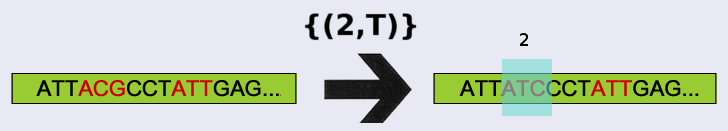
\includegraphics[scale=0.3]{images/ejemplo_mutation.png}\\       
      \end{center}
      \vspace{-0.1cm}
      Es importante notar que las mutantes obtenidas son resistentes a todos los antirretrovirales del conjunto de entrada.
    \end{block}       
}


\frame{
    \frametitle{Soluci\'on}
    \begin{block}{Generaci\'on del \'arbol}
      \begin{enumerate}
      \item \textbf {Tomar una secuencia en representaci\'on del virus y todos los antirretrovirales conocidos hasta el momento.}
      \item \textbf {Seleccionar los antirretrovirales que realmente pueden ser aplicados a la secuencia. De no haber ninguno aplicable, saltar al paso 7.}
      \item \textbf {Combinar los antirretrovirales seleccionados en el paso anterior.}
      \item \textbf {Aplicar cada combinaci\'on a la secuencia y obtener las secuencias mutantes.}
      \item \textbf {Calcular la FE de cada mutante.}
      \item Ejecutar este proceso para cada una de las mutantes obtenidas, luego, saltar al paso 8.
      \item Informar resultado.
      \item Terminar.
      \end{enumerate}
    \end{block}
}



\begin {frame}[fragile]
    \frametitle{Implementaci\'on - Predicci\'on de la Estructura Secundaria}
      Esta predicci\'on consiste en obtener la \emph{estructura secundaria} a partir de la estructura primaria. El m\'etodo utilizado se conoce bajo el nombre de \textbf{predicci\'on por \emph{minimal free energy (mfe)}}. El mismo, encuentra la estructura secundaria que minimiza la energ\'ia libre.\\
      \begin{block} {Ejemplo de una predicci\'on.}
      \scriptsize
      \begin{lstlisting}[basicstyle=\tt, frame=trBL, tabsize=4] 
	  combeng@fudepan:~$ RNAfold
	  Input string (upper or lower case); 
	  ....,....1....,....2....,....3....,....4...
	  AAAGGCAACGGCCAU
	  length = 15
	  AAAGGCAACGGCCAU
	  ...(((....)))..
	  minimum free energy =  -4.40 kcal/mol
      \end{lstlisting}
      \end{block}
      \normalsize
\end{frame}

\frame{
    \frametitle{Soluci\'on}
    \begin{block}{Generaci\'on del \'arbol}
      \begin{enumerate}
      \item \textbf {Tomar una secuencia en representaci\'on del virus y todos los antirretrovirales conocidos hasta el momento.}
      \item \textbf {Seleccionar los antirretrovirales que realmente pueden ser aplicados a la secuencia. De no haber ninguno aplicable, saltar al paso 7.}
      \item \textbf {Combinar los antirretrovirales seleccionados en el paso anterior.}
      \item \textbf {Aplicar cada combinaci\'on a la secuencia y obtener las secuencias mutantes.}
      \item \textbf {Calcular la FE de cada mutante.}
      \item \textbf {Ejecutar este proceso para cada una de las mutantes obtenidas, luego, saltar al paso 8.}
      \item \textbf{Informar resultado.}
      \item Terminar.
      \end{enumerate}
    \end{block}
}



\begin{frame}[fragile]
    \frametitle{Implementaci\'on - Datos de salida}
      La salida obtenida tras una ejecuci\'on de la aplicaci\'on, es un archivo conteniendo cada camino del \'arbol. Dicho de otra forma, el archivo contiene todas las terapias posibles, adem\'as de mostrar c\'omo fue variando la energ\'ia libre en cada paso de dichas terapias. Este archivo, es utilizado por R para generar los res\'umenes estad\'isticos necesarios (gr\'aficos, tendencias, etc).
\scriptsize
      \begin{lstlisting}[basicstyle=\tt, frame=trBL, tabsize=4] 
	...
	Therapy:  {5,6,7} -->  {16,17} -->  {13,15} -->  {10,12}
	FEs list: [-321 , -319.4 , -327.8 , -313.6 , -312.2 ]
	Therapy Length = 4
	Mutation: CCTCAGGTCACTCTTTGGCAACGACCCCTC .... 
	...
      \end{lstlisting}
    \normalsize
\end{frame}

\subsection{Resultados}
\frame{
    \frametitle{Resultados}
    \begin{block}{Promedio de Longitud de Terapia}
      Esta estad\'istica representa la cantidad de fallos virol\'ogicos que ocurrieron hasta que el virus se hizo resistente a todos los antirretrovirales. Dependiendo de c\'omo vaya mutando el virus, var\'ia la longitud de la terapia.
      \vspace{-0.3cm}
      \begin{center}
	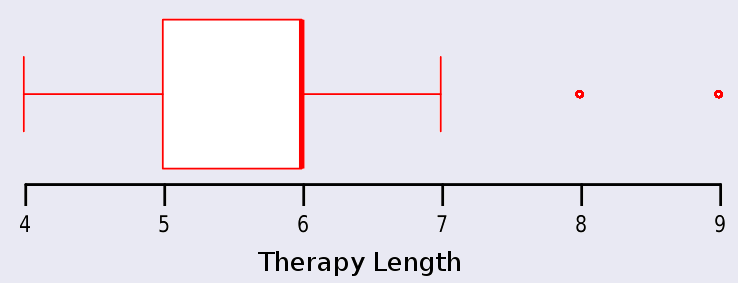
\includegraphics[scale=0.35]{images/therapy_length.png}\\       
      \end{center}
    \end{block}
}

\frame{
    \frametitle{Resultados}
    \begin{block}{Energ\'ia Libre de las mutantes en Relaci\'on a la Longitud de Terapia}
       Este resumen estad\'istico muestra c\'omo la energ\'ia libre de las mutantes se incrementa o decrementa acorde se avanza sobre la terapia.\\
      \begin{center}
	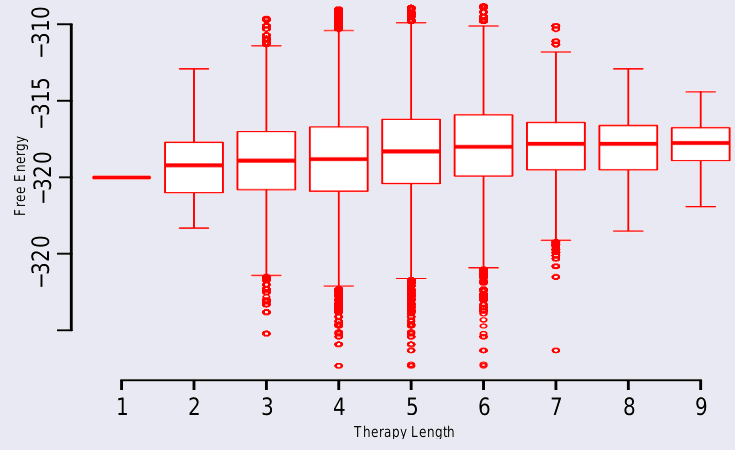
\includegraphics[scale=0.3]{images/free_energy_by_thrapy_length.png}\\       
      \end{center}
    \end{block}
}

\frame{
    \frametitle{Resultados}
    \begin{block}{Estimaci\'on de Tendencia de la Energ\'ia Libre}
       Este gr\'afico muestra informaci\'on acerca de la tendencia de la energ\'ia libre a medida que se avanza en la terapia.
      \begin{center}
	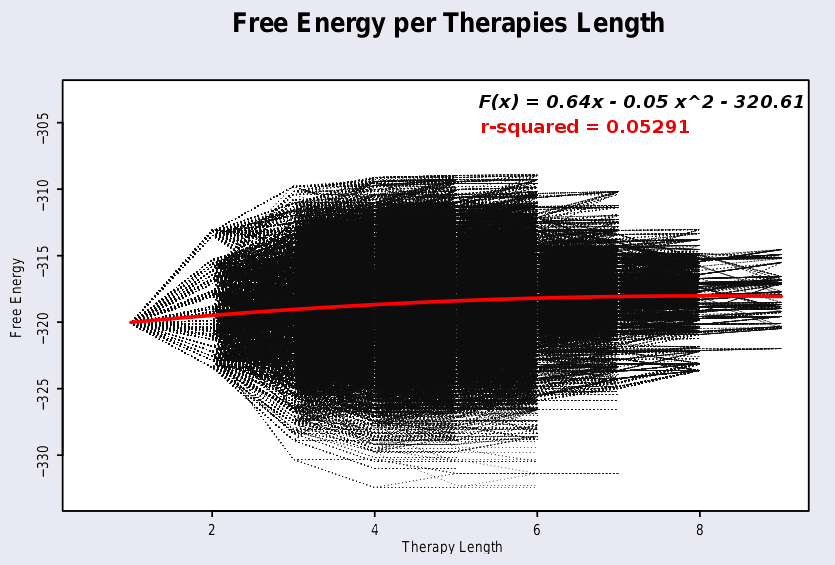
\includegraphics[scale=0.28]{images/ffe_vs_thLength.png}
      \end{center}
    \end{block}
}


\section{Conclusi\'on y trabajo futuro}
\subsection{Conclusi\'on}
\frame{
  \frametitle{Conclusi\'on}
  \begin{itemize}
    \item El motor combinatorio funciona correctamente, independientemente del problema que lo utilice.
    \item Correr la aplicaci\'on en ``modo completo'' es muy costoso. El \'arbol generado al armar todas las posibles terapias es muy grande.
    \item El presente trabajo nos ha permitido realizar una publicaci\'on.
    \item Nos vimos obligados a profundizar nuestros conocimientos en algunos aspectos que no est\'an cubiertos en la carrera.
  \end{itemize}
}

\subsection{Trabajo futuro}
\frame{
  \frametitle{Trabajo futuro}
  \begin{itemize}
    \item Correr la aplicaci\'on en ``modo completo'' en un cluster.
    \item Implementar nuevas pol\'iticas de combinaci\'on.
    \item Implementar nuevas pol\'iticas de poda, esto permitir\'a acotar de manera relevante el \'arbol de ejecuci\'on.
    \item Implementar las funcionalidades necesarias para hacer la aplicaci\'on independiente de la arquitectura.
    \item Implementar una interfaz gr\'afica para visualizar los resultados intuitivamente.
  \end{itemize}
  }

	\frame {
		\centerline{\Huge{\textbf{?`Preguntas?}}}
	}

	\frame {
		\centerline{\Huge{\textbf{Gracias}}}
	}
  
\end{document}
